\documentclass[11pt,a4paper]{article}

\usepackage[margin=1in]{geometry}
\usepackage[T1]{fontenc}
\usepackage[utf8]{inputenc}
\usepackage{lmodern}
\usepackage{amsmath,amssymb}
\usepackage{booktabs}
\usepackage{array}
\usepackage{longtable}
\usepackage{graphicx}
\usepackage{subcaption}
\usepackage{float}
\usepackage{xcolor}
\usepackage{hyperref}
\usepackage{enumitem}
\usepackage{verbatim}

\hypersetup{
  colorlinks=true,
  linkcolor=blue!60!black,
  urlcolor=blue!60!black,
  citecolor=blue!60!black
}

\setlist[itemize]{topsep=3pt,itemsep=3pt,leftmargin=18pt}
\setlength{\parskip}{4pt}
\setlength{\parindent}{0pt}

\newcommand{\T}{10{,}000}
\newcommand{\plot}[2]{
  \begin{figure}[H]
    \centering
    \includegraphics[width=0.82\textwidth]{assets/plots/#1}
    \caption{#2}
  \end{figure}
}

\title{Online Learning Applications Project}
\author{Mohammad Javad Zandiyeh (11044962)}
\date{\today}

\begin{document}

\maketitle
\tableofcontents
\newpage

\section{Introduction}

This report documents the implementation and empirical evaluation of an online
learning project for budget-constrained bidding in repeated first-price
auctions. The repository implements four progressively harder requirements:

\begin{itemize}
  \item Requirement 1: single-campaign stochastic bidding;
  \item Requirement 2: multi-campaign stochastic bidding with a global budget and
  conflict constraints;
  \item Requirement 3: a best-of-both-worlds primal-dual method that works in
  both stochastic and highly non-stationary environments;
  \item Requirement 4: piecewise-stationary bidding with sliding-window and
  change-detection extensions of Combinatorial-UCB.
\end{itemize}

The goal of the project is not only to run the algorithms, but to implement the
full pipeline: synthetic scenario generation, clairvoyant baselines, budget-safe
simulation, reproducible experiments, and diagnostic plots that explain both
successful and unexpected behaviors.

\section{Problem Formulation}

\subsection{Single-campaign setting}

At each round $t=1,\dots,T$, the learner chooses a bid $b_t$ from a discrete set
$\mathcal{B} \subset [0,1]$. The environment draws the highest competing bid
$m_t$, and the learner wins iff $b_t \ge m_t$. In a first-price auction,

\[
f_t(b_t) = (v - b_t)\mathbf{1}\{b_t \ge m_t\},
\qquad
c_t(b_t) = b_t \mathbf{1}\{b_t \ge m_t\},
\]

where $v$ is the campaign valuation. The learner has a finite budget $B$, so the
online policy must trade off utility maximization against pacing the spend over
time.

\subsection{Multi-campaign setting}

In the multi-campaign setting there are $N$ campaigns, one bid can be selected
per campaign, and all campaigns share a \emph{single global budget}. Two extra
constraints appear:

\begin{itemize}
  \item some campaigns cannot be activated together because of a conflict graph;
  \item feedback may be semi-bandit or full-information depending on the
  requirement.
\end{itemize}

The per-round budget target is denoted by $\rho = B/T$. The natural clairvoyant
benchmarks therefore optimize expected or empirical utility under the long-term
constraint $\mathbb{E}[c_t] \le \rho$.

\section{Implementation Overview}

\subsection{Repository structure}

The implementation is organized as follows:

\begin{verbatim}
src/ola/
  algorithms/
    ucb1.py
    ucb_budget.py
    combinatorial_ucb.py
    primal_dual.py
    nonstationary_ucb.py
    pacing.py
  auction.py
  baseline.py
  conflict_graph.py
  distributions.py
  environment.py
  metrics.py
  simulation.py

data/
  generate_datasets.py
  scenarios/*.json
  samples/*.csv

experiments/
  run_requirement1.py
  run_requirement2.py
  run_requirement3.py
  run_requirement4.py
\end{verbatim}

The code uses only a small scientific Python stack: \texttt{numpy},
\texttt{scipy}, \texttt{matplotlib}, and \texttt{networkx}. This keeps the
project lightweight while still supporting LP solving, random sampling, graph
operations, and figure generation.

\subsection{Central design choices}

Several implementation choices are shared by all requirements:

\begin{itemize}
  \item \textbf{Centralized budget bookkeeping.} Budget enforcement is implemented
  in \texttt{simulation.py}, not inside the bidders. This guarantees that all
  learners are evaluated under the same stopping rule.
  \item \textbf{Budget-safe termination.} In the single-campaign case the learner
  stops as soon as the remaining budget is below the maximum bid. In the
  multi-campaign case it stops when the remaining budget cannot cover the
  worst-case joint action, namely
  \[
  (\text{max independent set size}) \times (\text{max bid}).
  \]
  \item \textbf{Explicit baselines.} All regret curves are measured against
  clairvoyant benchmarks implemented in \texttt{baseline.py}, either from the
  true underlying distributions or from the realized non-stationary sequence.
  \item \textbf{Reproducibility.} The dataset generator writes JSON scenario files
  and reproducible sample CSVs. The experiment scripts fix the random seeds and
  write summary CSV files used by this report.
\end{itemize}

\subsection{Single-campaign optimization oracle}

For Requirement 1, the constrained bidding LP

\[
\max_{\gamma \in \Delta(\mathcal{B})} \sum_b \gamma(b)\,\bar f(b)
\quad
\text{s.t.}
\quad
\sum_b \gamma(b)\,\bar c(b)\le \rho
\]

is solved in closed form in \texttt{baseline.py}. Because the feasible region has
only the simplex constraint and one budget constraint, an optimal vertex is
supported on at most two bids. The implementation therefore enumerates feasible
pure bids and cost-straddling pairs rather than calling a generic LP solver.
This is both efficient and mathematically transparent.

\subsection{Multi-campaign optimization oracle}

For Requirements 2--4, the per-round oracle solves the combinatorial LP

\[
\max_x \sum_{i,b} f_{i}(b)x_{i,b}
\]

subject to:

\begin{itemize}
  \item at most one bid per campaign;
  \item total expected cost at most $\rho$;
  \item conflict constraints induced by the graph;
  \item non-negativity.
\end{itemize}

This oracle is implemented with \texttt{scipy.optimize.linprog}. The conflict
graphs used in the project are matchings (disjoint pairs), so the rounding
scheme in \texttt{combinatorial\_ucb.py} is exact for the intended setting:
free campaigns are Bernoulli-rounded independently, while conflict pairs are
rounded mutually exclusively.

\section{Datasets and Experimental Protocol}

\subsection{Synthetic scenarios}

All experiments use a common bid grid
\[
\mathcal{B} = \{0, 0.05, 0.10, \dots, 1.00\},
\]
with horizon $T=\T$. The dataset generator produces:

\begin{itemize}
  \item five single-campaign distributions: uniform, low competition, high
  competition, beta-skewed, and bimodal;
  \item three stationary multi-campaign scenarios: independent, conflict, and
  correlated;
  \item four non-stationary scenarios for Requirement 3:
  \texttt{ns\_abrupt}, \texttt{ns\_smooth}, \texttt{ns\_fast},
  \texttt{ns\_conflict};
  \item two dedicated piecewise-stationary scenarios for Requirement 4:
  \texttt{pw\_slight} and \texttt{pw\_frequent}, plus the reused abrupt and
  conflict cases.
\end{itemize}

The budget regimes are deliberately designed to stress the algorithms:

\begin{itemize}
  \item \textbf{Binding budget:} $\rho$ is set to half of the unconstrained
  expected or hindsight spend, so the constraint is genuinely active.
  \item \textbf{Slack budget:} the budget is large enough that the constraint is
  effectively inactive.
\end{itemize}

\subsection{Evaluation protocol}

The experiment scripts use the following protocol:

\begin{itemize}
  \item Requirement 1: 5 seeds;
  \item Requirement 2: 5 seeds;
  \item Requirement 3: 5 seeds for Primal-Dual and 3 seeds for
  Combinatorial-UCB;
  \item Requirement 4: 4 seeds, plus a smaller 2-seed window-sensitivity sweep.
\end{itemize}

The main outputs are regret curves, budget curves, diagnostic plots, and compact
CSV summaries. In the non-stationary setting, the report distinguishes between:

\begin{itemize}
  \item a \textbf{fixed hindsight optimum}, which is the correct benchmark for a
  best-of-both-worlds guarantee;
  \item a \textbf{dynamic optimum}, which can adapt to changes and is more
  appropriate for piecewise-stationary tracking.
\end{itemize}

\section{Requirement 1: Single-Campaign Stochastic Bidding}

\subsection{Implemented algorithms}

\paragraph{UCB1 baseline.}
The file \texttt{ucb1.py} implements standard UCB1 over the discrete bid set. It
uses realized auction utility as the arm reward and ignores the budget during
arm selection. This is a useful baseline because it is a valid no-regret method
when the budget is slack, but it has no built-in pacing mechanism.

\paragraph{Budgeted UCB.}
The file \texttt{ucb\_budget.py} implements a bandits-with-knapsacks style
learner. For each bid it maintains:

\[
f^{\text{UCB}}(b)=\hat f(b)+\text{radius}_f(b),
\qquad
c^{\text{LCB}}(b)=\hat c(b)-\text{radius}_c(b),
\]

then solves the constrained LP using optimistic utility and pessimistic cost.
Unseen bids are assigned maximal utility optimism and zero cost pessimism, which
forces exploration.

\subsection{Results summary}

\begin{table}[H]
\centering
\small
\begin{tabular}{lrrrrr}
\toprule
Scenario & $\rho$ & UCB1 util & UCB1 stop & Budgeted util & $T\cdot OPT$ \\
\midrule
\texttt{uniform\_binding} & 0.0800 & 346.5 & 3325 & 1020.9 & 1454.5 \\
\texttt{low\_competition\_binding} & 0.1630 & 1631.3 & 4812 & 3076.8 & 3672.3 \\
\texttt{high\_competition\_binding} & 0.2596 & 360.7 & 8854 & 336.9 & 862.4 \\
\texttt{beta\_skewed\_binding} & 0.1533 & 1109.3 & 4678 & 2153.5 & 2778.7 \\
\texttt{bimodal\_binding} & 0.0831 & 633.5 & 3140 & 1473.2 & 2286.0 \\
\bottomrule
\end{tabular}
\caption{Requirement 1 headline results on the binding-budget scenarios.}
\end{table}

The main pattern is clear: when the budget matters, ignoring it is expensive.
UCB1 tends to learn the unconstrained best bid, overspends early, and then earns
zero utility for the rest of the horizon. Budgeted UCB, instead, tracks the
per-round budget target and survives much longer.

The only notable exception is \texttt{high\_competition\_binding}, where the
budgeted learner slightly underperforms UCB1. This is an important result rather
than a failure to hide: when competition is strong, profitable wins are rare and
expensive, so the cautious cost pessimism of Budgeted UCB can make it overly
conservative in finite horizon. This is a good example of the remark
that unexpected results deserve discussion.

\begin{figure}[H]
\centering
\begin{subfigure}{0.48\textwidth}
  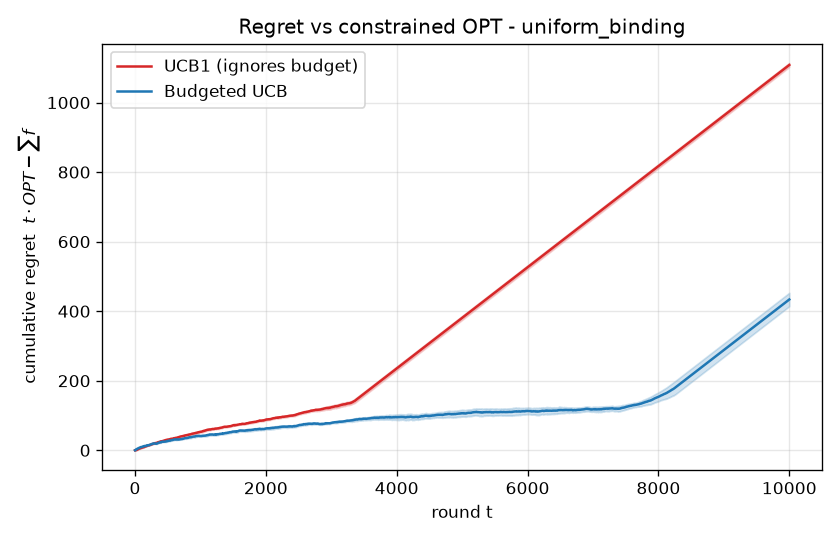
\includegraphics[width=\linewidth]{assets/plots/regret_uniform_binding.png}
  \caption{\texttt{uniform\_binding}}
\end{subfigure}
\hfill
\begin{subfigure}{0.48\textwidth}
  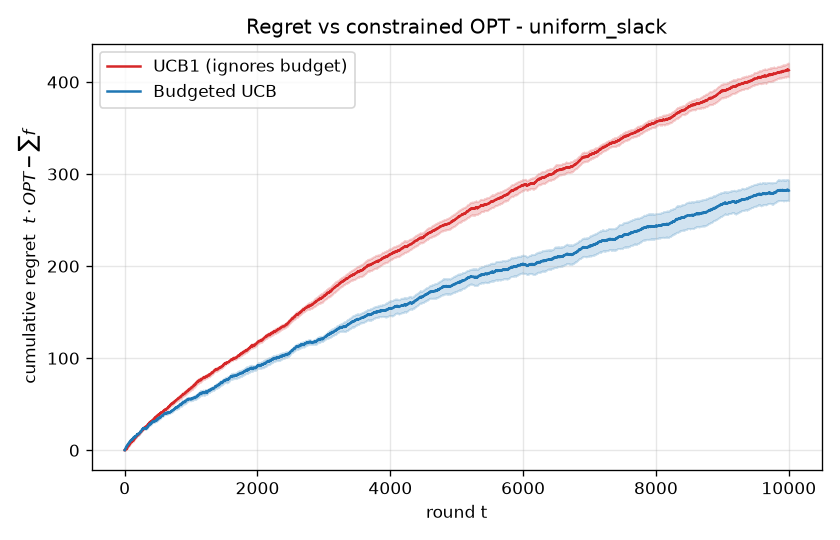
\includegraphics[width=\linewidth]{assets/plots/regret_uniform_slack.png}
  \caption{\texttt{uniform\_slack}}
\end{subfigure}
\caption{Representative Requirement 1 regret curves. Under a binding budget, UCB1
eventually depletes the budget and its regret becomes linear; under a slack
budget, both learners behave like valid no-regret stochastic bandits.}
\label{fig:req1-regret}
\end{figure}

\begin{figure}[H]
\centering
\begin{subfigure}{0.48\textwidth}
  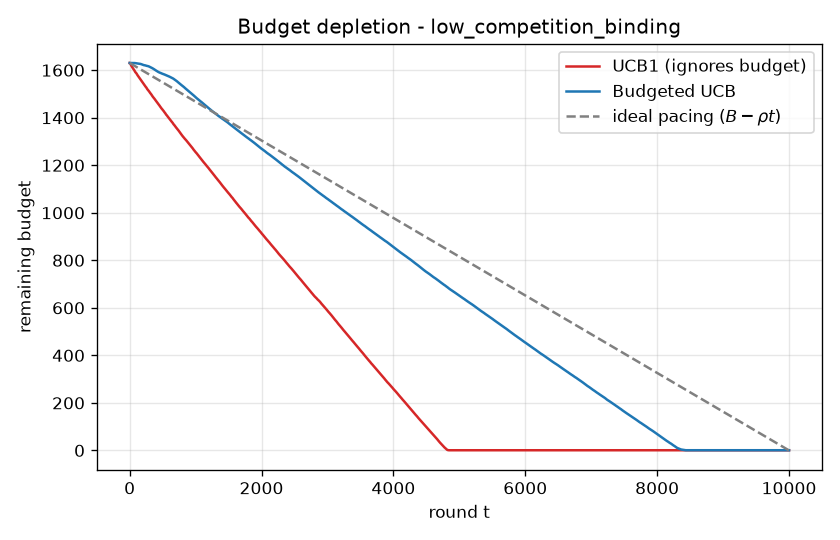
\includegraphics[width=\linewidth]{assets/plots/budget_low_competition_binding.png}
  \caption{Budget pacing}
\end{subfigure}
\hfill
\begin{subfigure}{0.48\textwidth}
  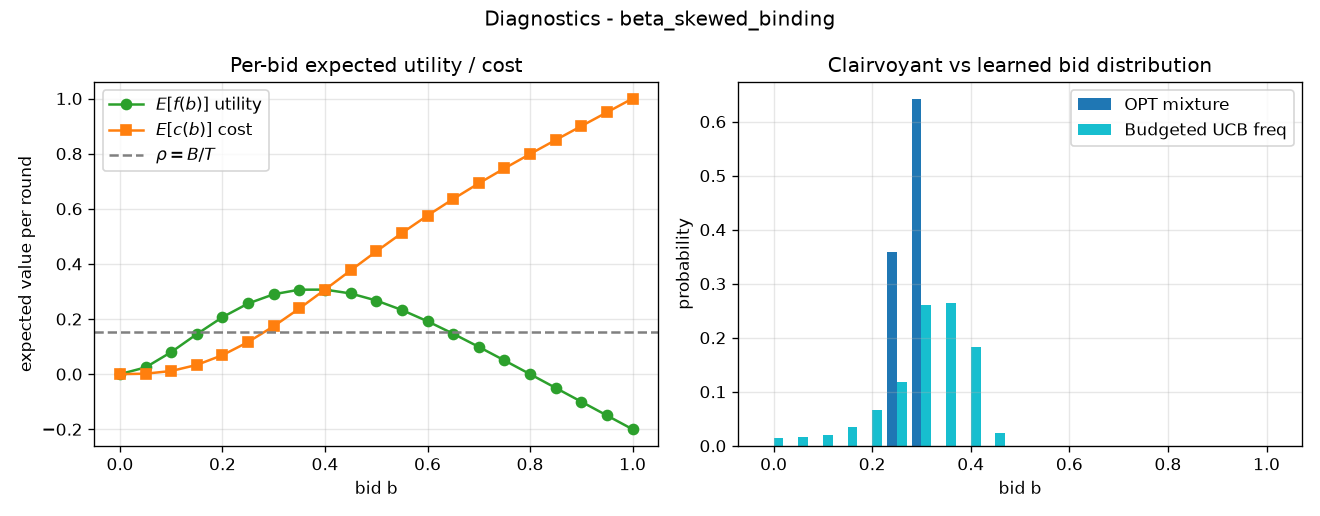
\includegraphics[width=\linewidth]{assets/plots/diagnostics_beta_skewed_binding.png}
  \caption{Learned bid distribution}
\end{subfigure}
\caption{Requirement 1 diagnostics: the budget-aware learner paces the spend and
learns a bid distribution close to the constrained clairvoyant optimum.}
\label{fig:req1-budget-diagnostics}
\end{figure}

\plot{scaling_regret.png}{Requirement 1 scaling experiment. The final regret of
Budgeted UCB grows approximately like $\sqrt{T}$, which is consistent with the
expected sublinear regret behavior.}

\subsection{Interpretation}

Requirement 1 validates the basic methodology of the project. The gap between
the two learners appears only when the constraint is active, exactly as theory
suggests. The additional diagnostic plots are especially useful because they
show that the improvement is not accidental: the budget-aware learner is not
just spending less, it is learning the correct \emph{mixture of bids}.

\section{Requirement 2: Multi-Campaign Stochastic Bidding}

\subsection{Implemented algorithm}

\texttt{combinatorial\_ucb.py} extends Requirement 1 to multiple simultaneous
campaigns. Each pair $(i,b)$ is treated as an arm, the confidence bounds are
computed per arm, and a linear optimization oracle chooses the best feasible
superarm under:

\begin{itemize}
  \item one bid per campaign,
  \item a global budget constraint,
  \item conflict-graph constraints.
\end{itemize}

The learner receives semi-bandit feedback, so only played campaign-bid pairs are
updated.

\subsection{Results summary}

\begin{table}[H]
\centering
\small
\begin{tabular}{lrrrrr}
\toprule
Scenario & $N$ & corr & $\rho$ & Comb-UCB util & $T\cdot OPT$ \\
\midrule
\texttt{multi\_independent\_binding} & 3 & 0.0 & 0.5027 & 5652.8 & 6350.1 \\
\texttt{multi\_conflict\_binding} & 4 & 0.0 & 0.3527 & 4315.6 & 5302.0 \\
\texttt{multi\_correlated\_binding} & 3 & 0.6 & 0.3164 & 4567.6 & 6713.1 \\
\bottomrule
\end{tabular}
\caption{Requirement 2 results on the binding-budget scenarios.}
\end{table}

The algorithm performs well across all three stationary multi-campaign regimes.
The summary CSV shows that the realized utility stays reasonably close to the
clairvoyant benchmark, the budget is respected, and the diagnostics show that
the empirical bid allocation concentrates on the oracle allocation.

The conflict case is particularly important because it validates the rounding
logic: the algorithm learns to drop the lower-value campaign in each conflict
pair, which is exactly the qualitative behavior expected from the oracle.

\begin{figure}[H]
\centering
\begin{subfigure}{0.48\textwidth}
  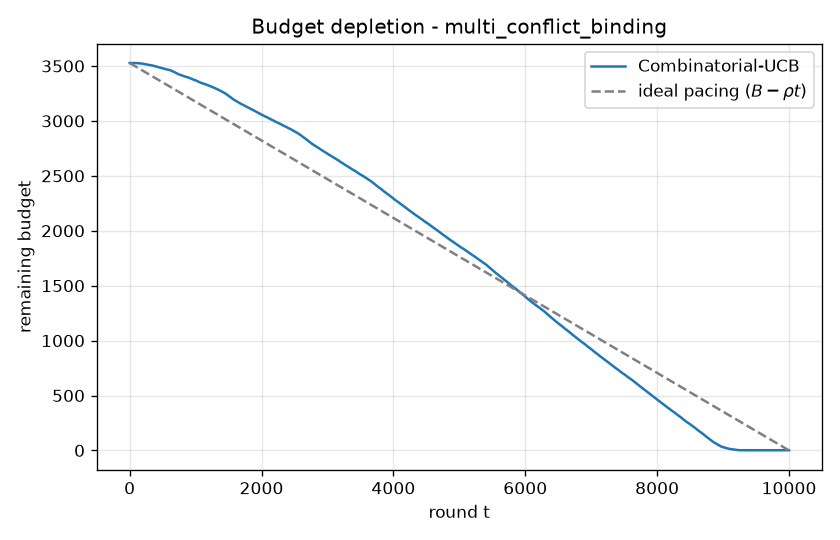
\includegraphics[width=\linewidth]{assets/plots/budget_multi_conflict_binding.png}
  \caption{Budget pacing}
\end{subfigure}
\hfill
\begin{subfigure}{0.48\textwidth}
  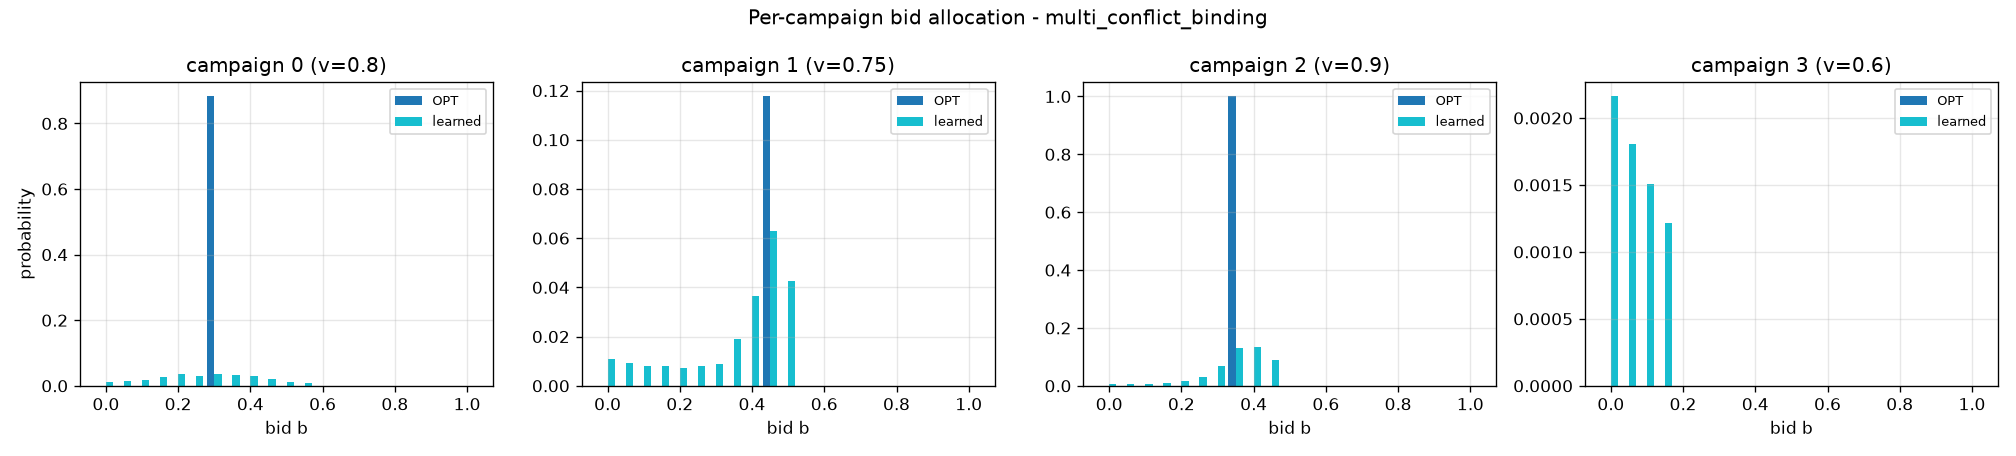
\includegraphics[width=\linewidth]{assets/plots/diagnostics_multi_conflict_binding.png}
  \caption{Conflict-aware allocation}
\end{subfigure}
\caption{Requirement 2 diagnostics. The learner both respects the global budget
and recovers the correct campaign-level allocation in the presence of conflicts.}
\label{fig:req2-budget-diagnostics}
\end{figure}

\plot{scaling_regret_multi.png}{Requirement 2 scaling experiment. The final
regret again follows an approximately $\sqrt{T}$ trend.}

Note that the final repository plot bundle reuses the filenames
\texttt{regret\_multi\_*} inside Requirement 3 for the direct Primal-Dual vs
Combinatorial-UCB comparison. For that reason, the unique Requirement 2 visual
evidence in this report is the budget, diagnostic, and scaling plots, while the
stationary regret numbers are taken from \texttt{summary\_req2.csv}.

\subsection{Interpretation}

Requirement 2 shows that the project is not merely a single-bandit simulation.
The implementation successfully combines budgeted exploration, graph-constrained
feasibility, and joint action rounding. Correlation makes the environment harder,
but the structure of the benchmark is still recovered because expected utility
and cost depend only on the marginal bid distributions.

\section{Requirement 3: Best-of-Both-Worlds Primal-Dual Learning}

\subsection{Implemented algorithm}

The key contribution of Requirement 3 is \texttt{PrimalDualBidder}. It combines:

\begin{itemize}
  \item a single dual variable $\lambda_t$ that prices the shared budget;
  \item a primal full-information learner based on Hedge;
  \item a factorization of the feasible action space into independent blocks
  induced by the matching conflict graph.
\end{itemize}

Given $\lambda_t$, each bid receives Lagrangian reward
\[
L_{i,t}(b) = f_{i,t}(b) - \lambda_t c_{i,t}(b).
\]

After observing the full vector of competing bids, the algorithm can score every
counterfactual action and update Hedge on each block. The dual variable is then
updated via projected online gradient descent:

\[
\lambda_{t+1}
=
\Pi_{[0,1/\rho]}
\left(\lambda_t + \eta_{\text{dual}}(\widehat c_t - \rho)\right).
\]

This design is precisely what makes the algorithm work in both stochastic and
non-stationary environments: unlike UCB, Hedge never collapses exploration, and
the budget is handled by the dual signal rather than by confidence bounds alone.

\subsection{Results summary}

\begin{table}[H]
\centering
\scriptsize
\begin{tabular}{l l r r r r}
\toprule
Scenario & World & $T\!\cdot\!OPT_{\text{fixed}}$ & $T\!\cdot\!OPT_{\text{dyn}}$ & PD regret & CUCB regret \\
\midrule
\texttt{ns\_abrupt\_binding} & non-stationary & 5677.3 & 6283.0 & 689.9 & 222.1 \\
\texttt{ns\_smooth\_binding} & non-stationary & 5327.9 & 5375.9 & 1455.8 & 1909.7 \\
\texttt{ns\_fast\_binding} & non-stationary & 5510.7 & 5844.2 & 511.5 & 1172.9 \\
\texttt{ns\_conflict\_binding} & non-stationary & 3588.7 & 4667.2 & 438.9 & 522.4 \\
\texttt{multi\_independent\_binding} & stochastic & 6350.1 & 6350.1 & 430.8 & 699.7 \\
\texttt{multi\_conflict\_binding} & stochastic & 5302.0 & 5302.0 & 405.2 & 1024.2 \\
\texttt{multi\_correlated\_binding} & stochastic & 6713.1 & 6713.1 & 734.1 & 2153.6 \\
\bottomrule
\end{tabular}
\caption{Requirement 3 comparison against the best fixed feasible policy in
hindsight. The dynamic optimum is reported to quantify the price of
non-stationarity.}
\end{table}

This is the strongest section of the project. The same primal-dual learner is
competitive in both worlds, while Combinatorial-UCB degrades badly whenever its
stationarity assumptions become stale. On \texttt{ns\_fast\_binding}, for
instance, the primal-dual regret is less than half the UCB-style regret.

At the same time, the results are nuanced rather than uniformly one-sided:
\texttt{ns\_abrupt\_binding} is a case where Combinatorial-UCB still beats the
primal-dual method with respect to the \emph{fixed} benchmark. This is worth
highlighting: best-of-both-worlds does not mean domination on every instance,
only robustness across regimes. The project therefore correctly surfaces the
trade-off instead of overselling the algorithm.

\plot{bobw_summary.png}{Requirement 3 summary plot. The primal-dual algorithm is
consistently strong across stochastic and non-stationary regimes, while the
stochastic-only baseline becomes unreliable when the environment changes.}

\begin{figure}[H]
\centering
\begin{subfigure}{0.48\textwidth}
  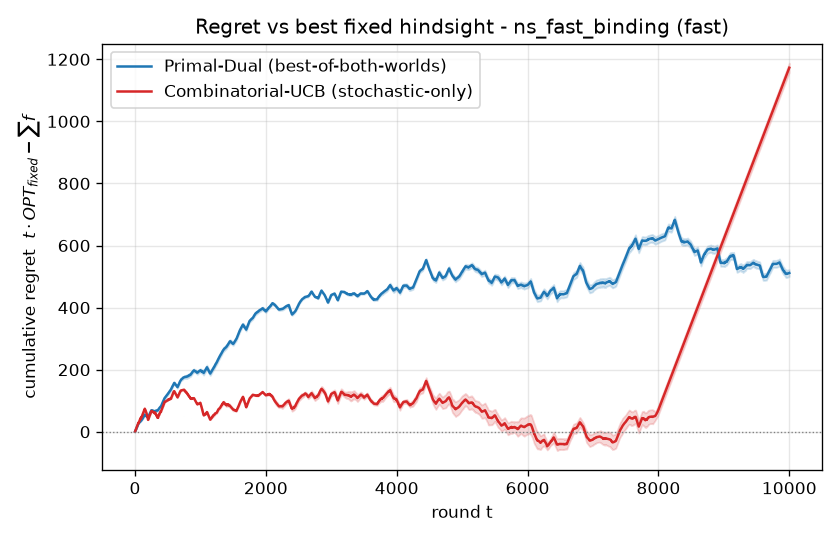
\includegraphics[width=\linewidth]{assets/plots/regret_ns_fast_binding.png}
  \caption{\texttt{ns\_fast\_binding}}
\end{subfigure}
\hfill
\begin{subfigure}{0.48\textwidth}
  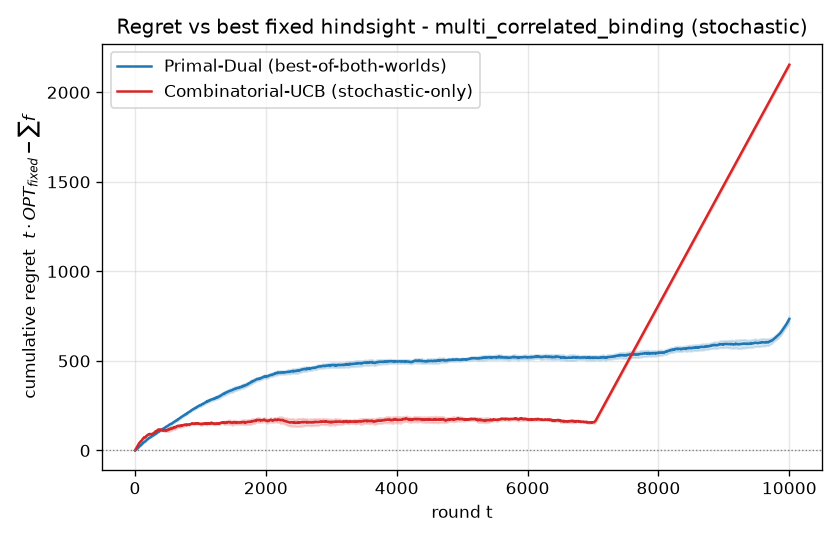
\includegraphics[width=\linewidth]{assets/plots/regret_multi_correlated_binding.png}
  \caption{\texttt{multi\_correlated\_binding}}
\end{subfigure}
\caption{Representative Requirement 3 regret curves. The primal-dual learner
remains competitive both in a highly non-stationary regime and in the reused
stationary stochastic regime.}
\label{fig:req3-regret}
\end{figure}

\begin{figure}[H]
\centering
\begin{subfigure}{0.48\textwidth}
  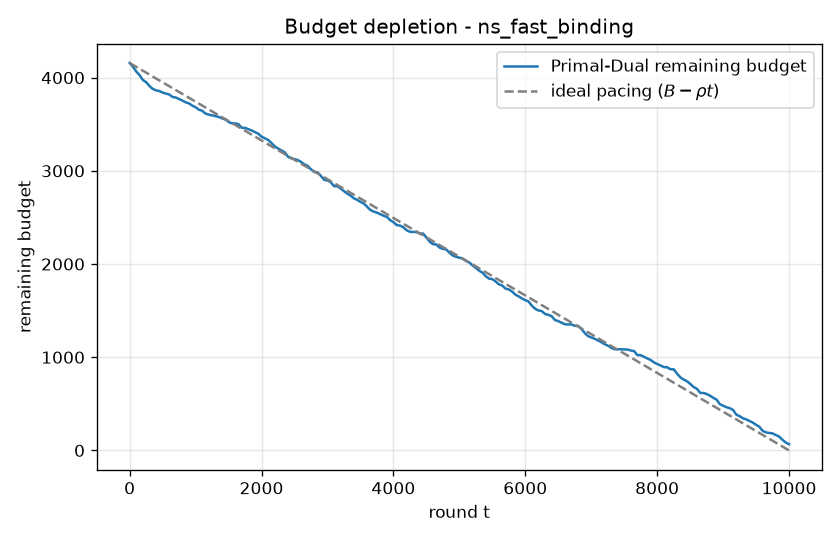
\includegraphics[width=\linewidth]{assets/plots/budget_ns_fast_binding.png}
  \caption{Budget pacing}
\end{subfigure}
\hfill
\begin{subfigure}{0.48\textwidth}
  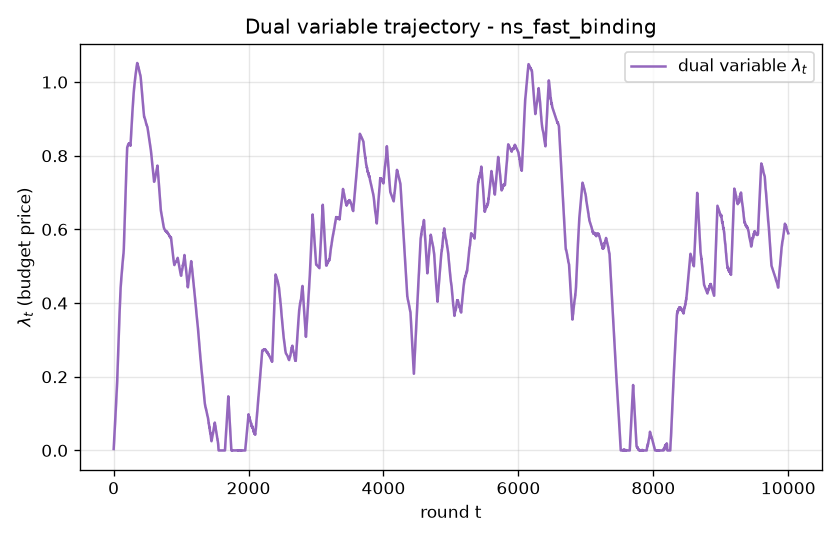
\includegraphics[width=\linewidth]{assets/plots/dual_ns_fast_binding.png}
  \caption{Dual trajectory}
\end{subfigure}
\caption{Requirement 3 diagnostics on \texttt{ns\_fast\_binding}. The dual
variable acts as a real-time budget price, allowing the learner to react to
changing competition while pacing the spend until the horizon.}
\label{fig:req3-budget-dual}
\end{figure}

\plot{scaling_regret_pd.png}{Requirement 3 scaling experiment on the fast
non-stationary scenario. The final regret remains compatible with a sublinear
trend.}

\subsection{Interpretation}

The most convincing evidence for the primal-dual design is the \emph{shape} of
the curves. When Combinatorial-UCB fails, it usually fails in the same way:
confidence bounds become stale, the algorithm overspends early, and once the
budget is exhausted the regret turns into an almost linear ramp. The primal-dual
learner avoids this failure mode because it keeps updating on full feedback and
uses the dual variable to explicitly control pacing.

\section{Requirement 4: Piecewise-Stationary Learning}

\subsection{Implemented algorithms}

Requirement 4 extends Combinatorial-UCB in two classic ways:

\begin{itemize}
  \item \textbf{SlidingWindowCombinatorialUCBBidder:} only the last $W$
  observations of each arm are kept. The default implementation uses
  $W \approx 20\sqrt{T}$, larger than the textbook $\sqrt{T}$ rule because the
  combinatorial setting spreads samples over many arms.
  \item \textbf{ChangeDetectionCombinatorialUCBBidder:} each arm is equipped with
  a CUSUM detector with parameters
  \texttt{cusum\_m = 50}, \texttt{cusum\_eps = 0.15},
  \texttt{cusum\_h = 5.0}, and exploration probability
  \texttt{alpha = 0.01}.
\end{itemize}

These are compared against the original Comb-UCB and the Requirement 3
Primal-Dual method.

\subsection{Results summary}

\begin{table}[H]
\centering
\small
\begin{tabular}{lrrrrr}
\toprule
Scenario & $T\!\cdot\!OPT_{\text{dyn}}$ & Comb-UCB & SW-CombUCB & CD-CombUCB & Primal-Dual \\
\midrule
\texttt{pw\_slight\_binding} & 6822.9 & 1622.2 & \textbf{943.8} & 1805.2 & 1050.7 \\
\texttt{ns\_conflict\_binding} & 4659.6 & 1576.5 & 1553.3 & 1688.4 & \textbf{1513.3} \\
\texttt{ns\_abrupt\_binding} & 6267.2 & \textbf{867.5} & 1350.9 & 1070.9 & 1281.1 \\
\texttt{pw\_frequent\_binding} & 5413.0 & \textbf{748.2} & 784.4 & 1489.4 & 985.7 \\
\bottomrule
\end{tabular}
\caption{Requirement 4 final regrets against the dynamic per-interval optimum.}
\end{table}

This requirement is interesting precisely because there is no universal winner.
The results clearly show the price of robustness:

\begin{itemize}
  \item SW-CombUCB wins when changes are relatively infrequent and the budget is
  tight (\texttt{pw\_slight\_binding});
  \item Primal-Dual is strongest in the conflict-heavy budget-sensitive case
  (\texttt{ns\_conflict\_binding});
  \item plain Comb-UCB is still hard to beat when the environment is not too far
  from stationary (\texttt{ns\_abrupt\_binding}, \texttt{pw\_frequent\_binding});
  \item CD-CombUCB is the most sensitive method and performs poorly when resets
  and forced exploration consume too much of the budget.
\end{itemize}

\plot{req4_summary.png}{Requirement 4 summary comparison. The best method depends
on the frequency of changes and on how expensive budget mistakes are.}

\begin{figure}[H]
\centering
\begin{subfigure}{0.48\textwidth}
  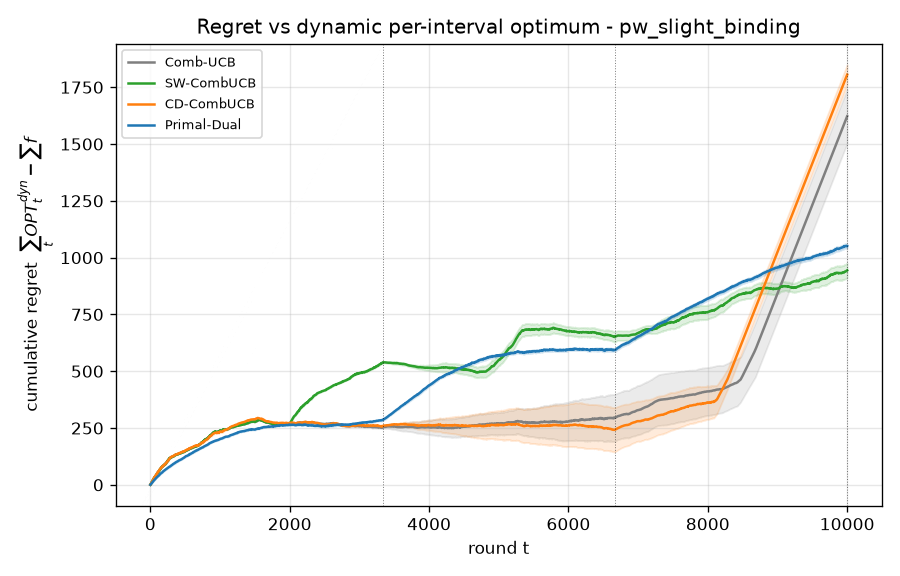
\includegraphics[width=\linewidth]{assets/plots/regret_req4_pw_slight_binding.png}
  \caption{\texttt{pw\_slight\_binding}}
\end{subfigure}
\hfill
\begin{subfigure}{0.48\textwidth}
  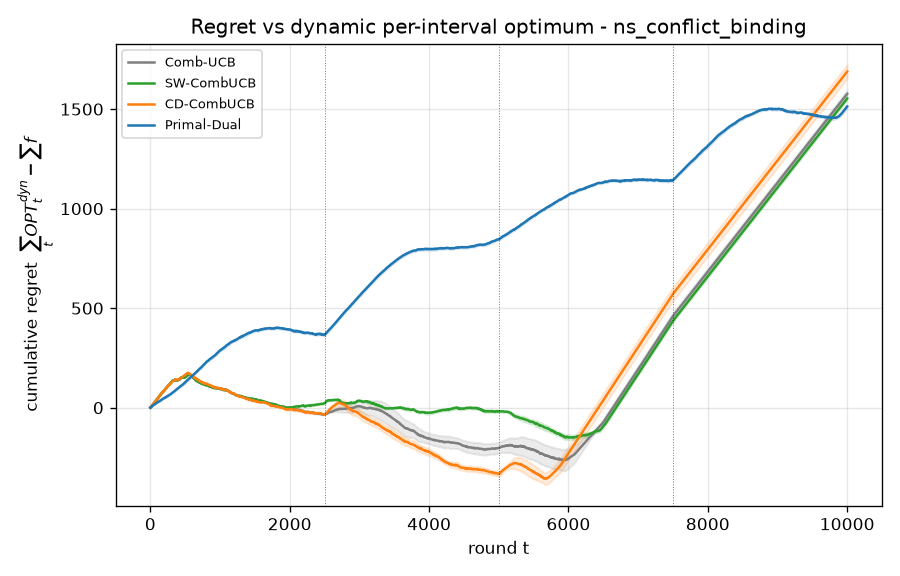
\includegraphics[width=\linewidth]{assets/plots/regret_req4_ns_conflict_binding.png}
  \caption{\texttt{ns\_conflict\_binding}}
\end{subfigure}
\caption{Requirement 4 regret curves against the dynamic benchmark.}
\label{fig:req4-regret}
\end{figure}

\begin{figure}[H]
\centering
\begin{subfigure}{0.48\textwidth}
  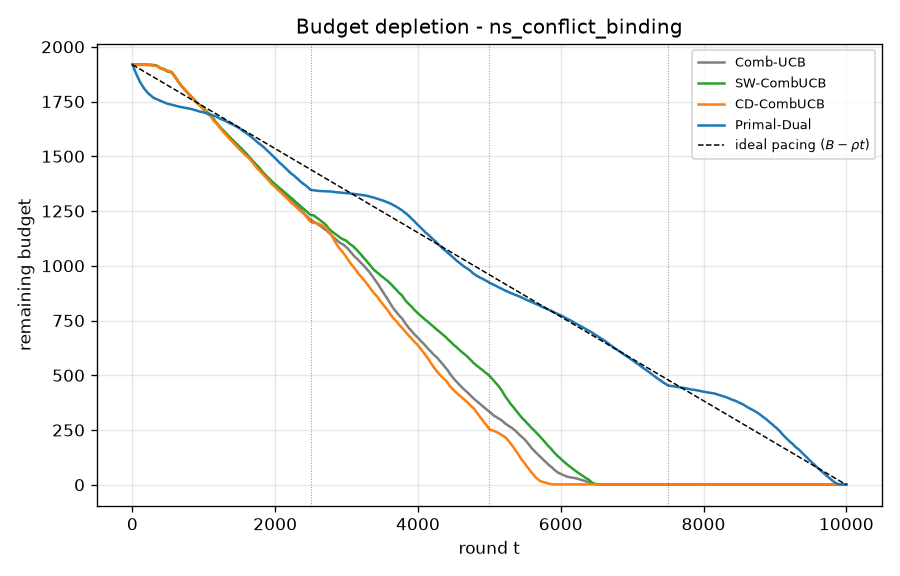
\includegraphics[width=\linewidth]{assets/plots/budget_req4_ns_conflict_binding.png}
  \caption{Budget trajectories}
\end{subfigure}
\hfill
\begin{subfigure}{0.48\textwidth}
  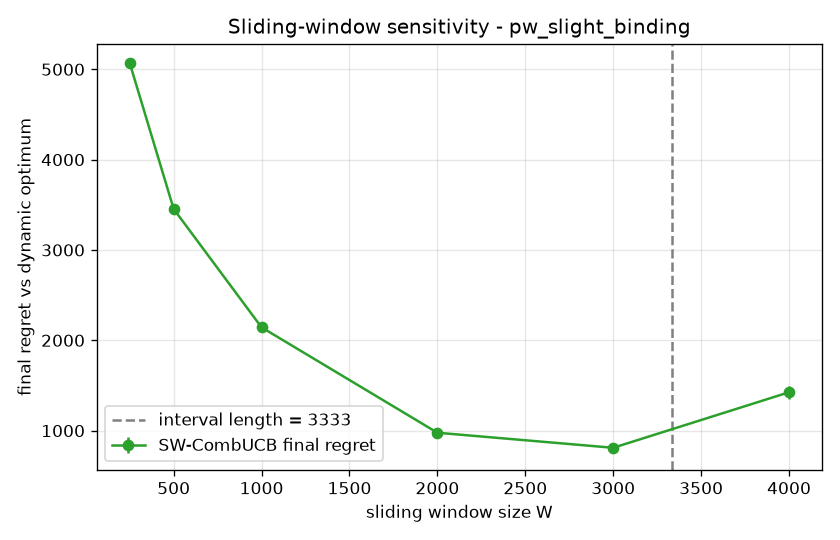
\includegraphics[width=\linewidth]{assets/plots/window_sensitivity.png}
  \caption{Sensitivity to the window size}
\end{subfigure}
\caption{Requirement 4 diagnostics. The conflict scenario highlights the value
of primal-dual pacing, while the window sweep shows that the best $W$ depends on
the unknown interval length.}
\label{fig:req4-budget-window}
\end{figure}

\subsection{Interpretation}

The project correctly captures a subtle point from the course: non-stationary
methods can pay an unnecessary price when the world is close to stationary. This
is why Comb-UCB remains competitive in some piecewise-stationary instances. The
report should therefore not frame Requirement 4 as ``newer algorithms always win'';
instead, the correct conclusion is that adaptation mechanisms help only when
their bias-variance trade-off matches the change frequency.

\section{Cross-Cutting Discussion of Unexpected Results}

Several findings deserve explicit discussion:

\begin{enumerate}
  \item \textbf{Budget-aware learning is not always better in finite horizon.}
  The \texttt{high\_competition\_binding} scenario in Requirement 1 shows that
  stronger budget discipline can be too conservative when profitable wins are
  already scarce.

  \item \textbf{Best-of-both-worlds does not imply pointwise dominance.}
  In Requirement 3, the primal-dual method is the most robust overall, but it
  does not beat Combinatorial-UCB on every single instance. The
  \texttt{ns\_abrupt\_binding} scenario is the clearest counterexample.

  \item \textbf{Dynamic and fixed benchmarks tell different stories.}
  The large gap between $T\cdot OPT_{\text{fixed}}$ and
  $T\cdot OPT_{\text{dyn}}$ on scenarios such as
  \texttt{ns\_conflict\_binding} quantifies how much value is lost by insisting
  on a fixed action distribution in a changing environment.

  \item \textbf{Change detection is fragile under budget constraints.}
  Resets and forced exploration are expensive when the budget is binding. This is
  why CD-CombUCB is often the weakest method in Requirement 4 despite being more
  adaptive in principle.
\end{enumerate}

These are useful points for the oral presentation because they show a real
understanding of the algorithms, not just a list of plots.

\section{Conclusion}

The project delivers a coherent implementation of budget-constrained bidding
across stochastic, combinatorial, and non-stationary regimes. The strongest
engineering aspects are:

\begin{itemize}
  \item a clean separation between learning logic, simulation logic, and
  clairvoyant baselines;
  \item scenario generators that produce interpretable and reproducible instances;
  \item experiment scripts that are self-contained and produce both headline
  summaries and detailed diagnostics;
  \item careful comparison against the right benchmark for each requirement.
\end{itemize}

Empirically, the report supports four main conclusions:

\begin{itemize}
  \item budget-aware learning matters as soon as the budget truly binds;
  \item combinatorial structure and conflicts can be handled effectively through
  an LP oracle and structured rounding;
  \item the primal-dual approach is the most robust method across stochastic and
  rapidly changing environments;
  \item no non-stationary method dominates universally, and the degree of
  non-stationarity strongly affects which algorithm is preferable.
\end{itemize}

\appendix

\section{Complete Plot Gallery}

This appendix includes every generated figure copied into the report directory.
The main body focused on the most informative plots; the appendix preserves the
full experimental record.

\subsection{Requirement 1: all plots}

\begin{figure}[p]
\centering
\begin{subfigure}{0.48\textwidth}
  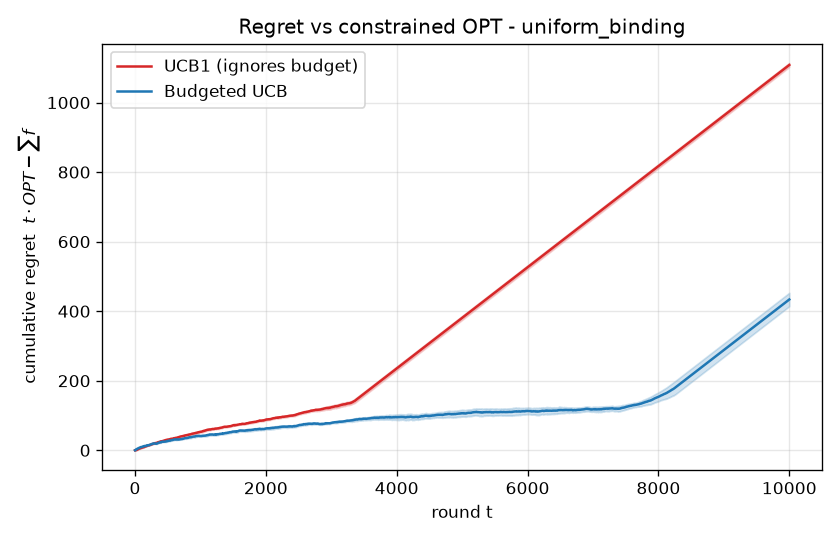
\includegraphics[width=\linewidth]{assets/plots/regret_uniform_binding.png}
  \caption{\texttt{uniform\_binding}}
\end{subfigure}
\hfill
\begin{subfigure}{0.48\textwidth}
  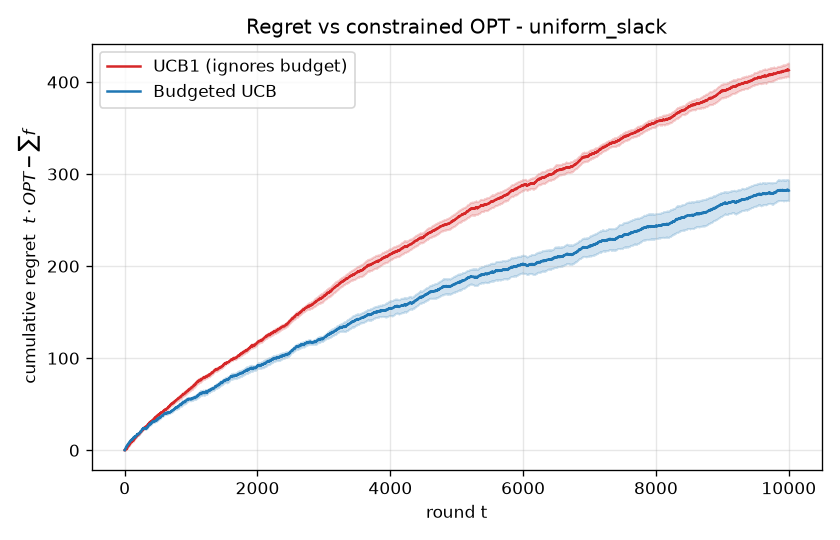
\includegraphics[width=\linewidth]{assets/plots/regret_uniform_slack.png}
  \caption{\texttt{uniform\_slack}}
\end{subfigure}
\caption{Requirement 1 regret plots: uniform scenario.}
\end{figure}

\begin{figure}[p]
\centering
\begin{subfigure}{0.48\textwidth}
  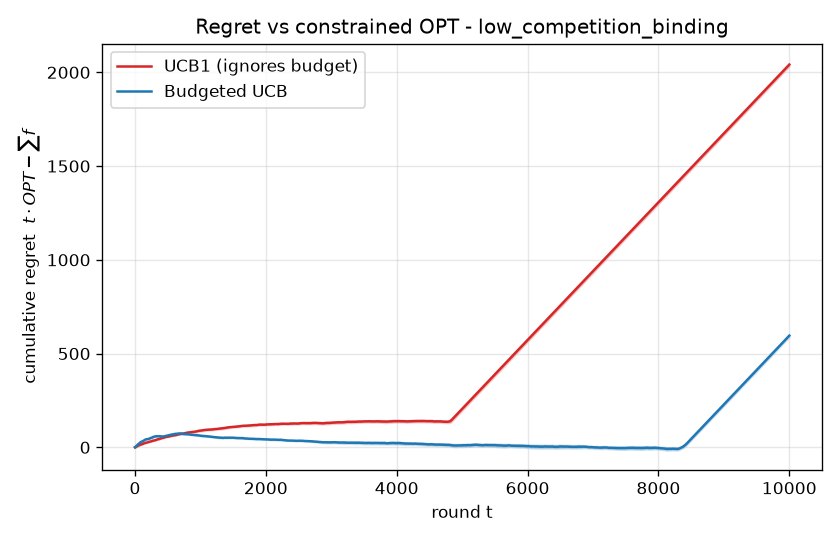
\includegraphics[width=\linewidth]{assets/plots/regret_low_competition_binding.png}
  \caption{\texttt{low\_competition\_binding}}
\end{subfigure}
\hfill
\begin{subfigure}{0.48\textwidth}
  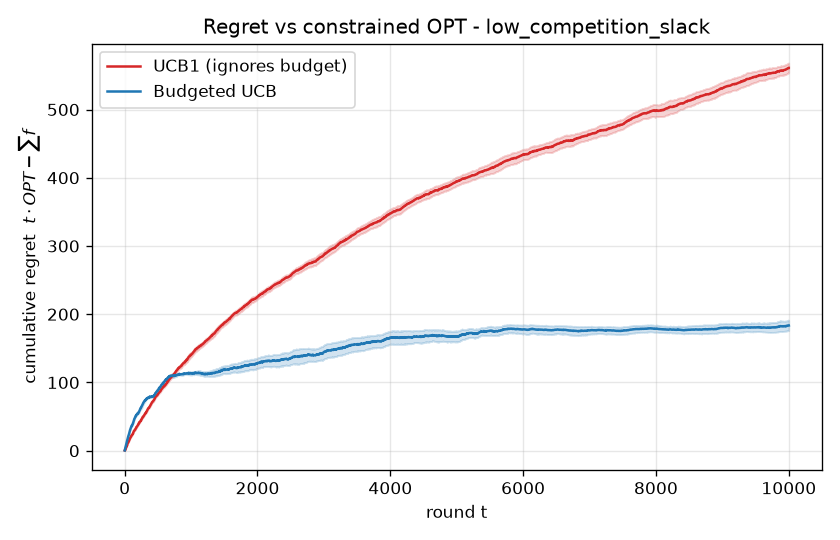
\includegraphics[width=\linewidth]{assets/plots/regret_low_competition_slack.png}
  \caption{\texttt{low\_competition\_slack}}
\end{subfigure}
\caption{Requirement 1 regret plots: low-competition scenario.}
\end{figure}

\begin{figure}[p]
\centering
\begin{subfigure}{0.48\textwidth}
  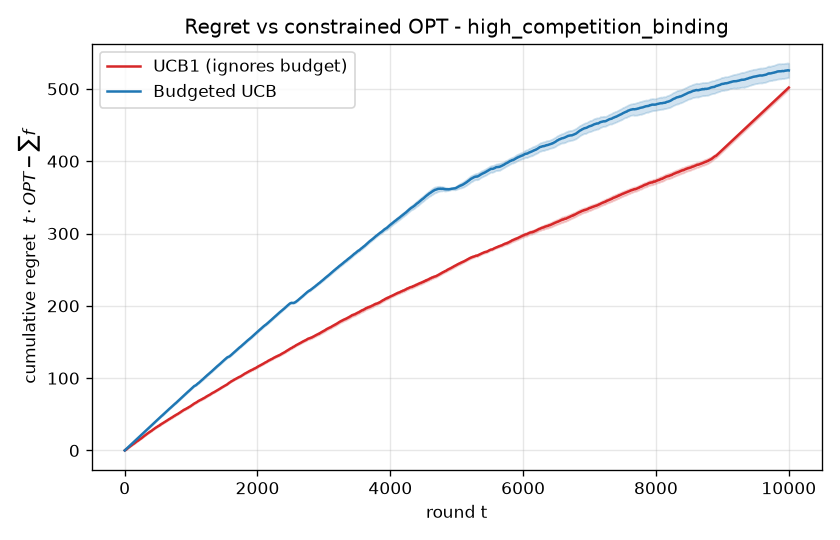
\includegraphics[width=\linewidth]{assets/plots/regret_high_competition_binding.png}
  \caption{\texttt{high\_competition\_binding}}
\end{subfigure}
\hfill
\begin{subfigure}{0.48\textwidth}
  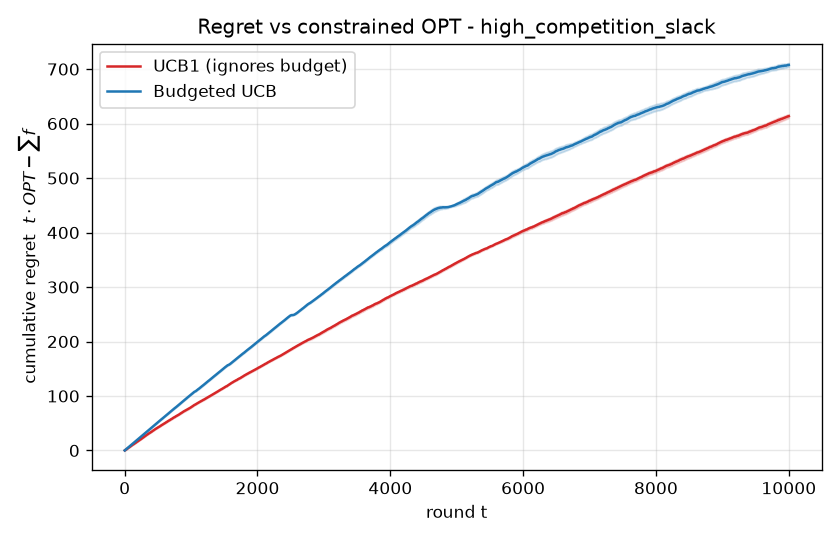
\includegraphics[width=\linewidth]{assets/plots/regret_high_competition_slack.png}
  \caption{\texttt{high\_competition\_slack}}
\end{subfigure}
\caption{Requirement 1 regret plots: high-competition scenario.}
\end{figure}

\begin{figure}[p]
\centering
\begin{subfigure}{0.48\textwidth}
  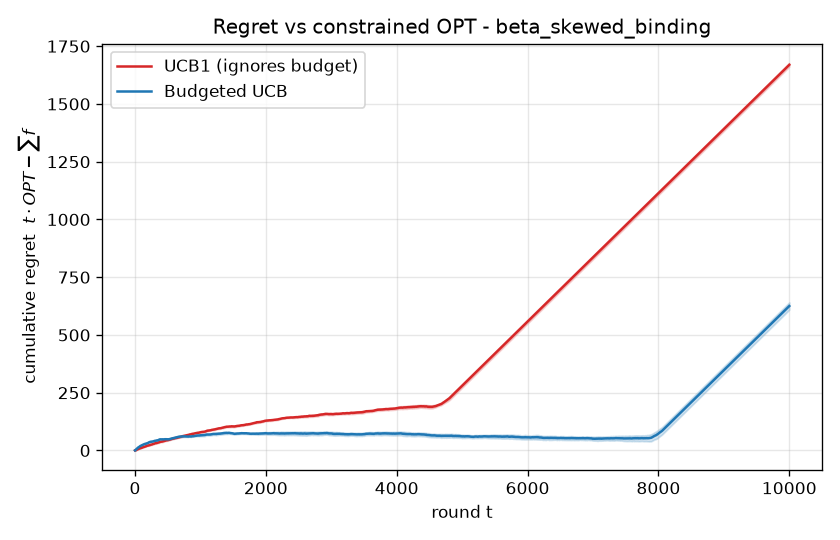
\includegraphics[width=\linewidth]{assets/plots/regret_beta_skewed_binding.png}
  \caption{\texttt{beta\_skewed\_binding}}
\end{subfigure}
\hfill
\begin{subfigure}{0.48\textwidth}
  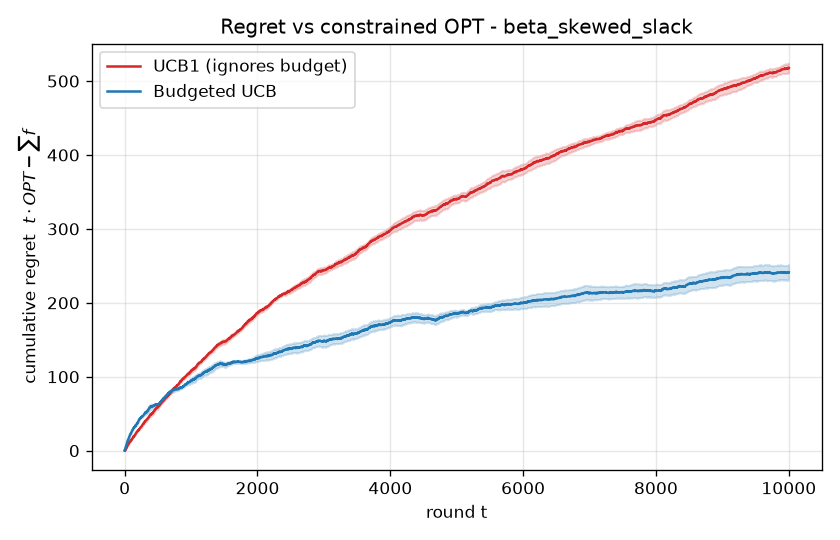
\includegraphics[width=\linewidth]{assets/plots/regret_beta_skewed_slack.png}
  \caption{\texttt{beta\_skewed\_slack}}
\end{subfigure}
\caption{Requirement 1 regret plots: beta-skewed scenario.}
\end{figure}

\begin{figure}[p]
\centering
\begin{subfigure}{0.48\textwidth}
  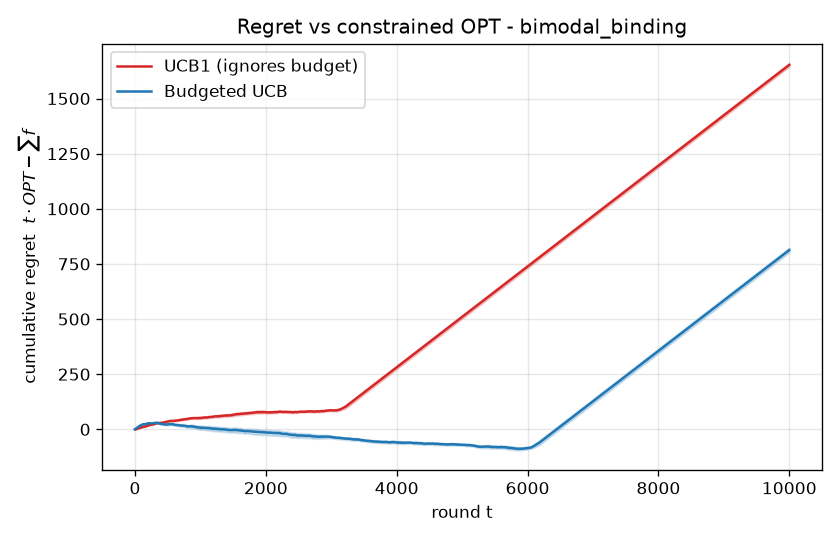
\includegraphics[width=\linewidth]{assets/plots/regret_bimodal_binding.png}
  \caption{\texttt{bimodal\_binding}}
\end{subfigure}
\hfill
\begin{subfigure}{0.48\textwidth}
  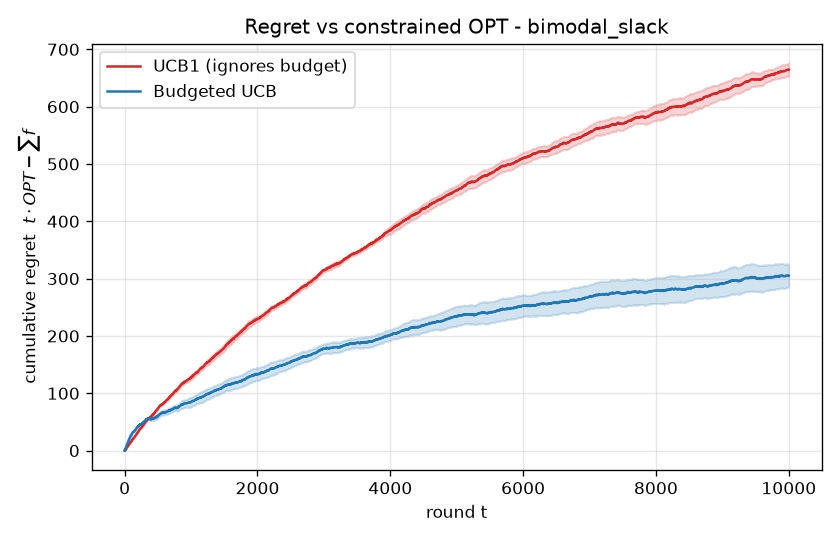
\includegraphics[width=\linewidth]{assets/plots/regret_bimodal_slack.png}
  \caption{\texttt{bimodal\_slack}}
\end{subfigure}
\caption{Requirement 1 regret plots: bimodal scenario.}
\end{figure}

\begin{figure}[p]
\centering
\begin{subfigure}{0.48\textwidth}
  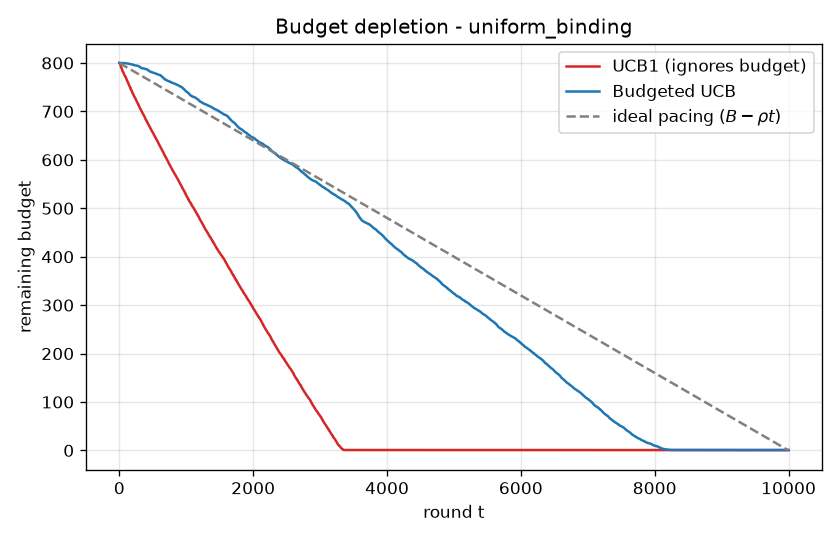
\includegraphics[width=\linewidth]{assets/plots/budget_uniform_binding.png}
  \caption{\texttt{uniform\_binding}}
\end{subfigure}
\hfill
\begin{subfigure}{0.48\textwidth}
  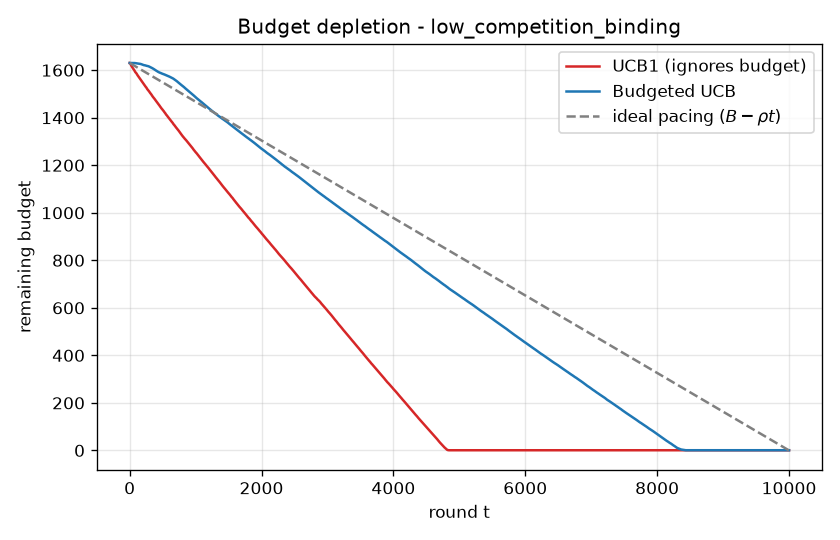
\includegraphics[width=\linewidth]{assets/plots/budget_low_competition_binding.png}
  \caption{\texttt{low\_competition\_binding}}
\end{subfigure}
\caption{Requirement 1 budget plots, part I.}
\end{figure}

\begin{figure}[p]
\centering
\begin{subfigure}{0.48\textwidth}
  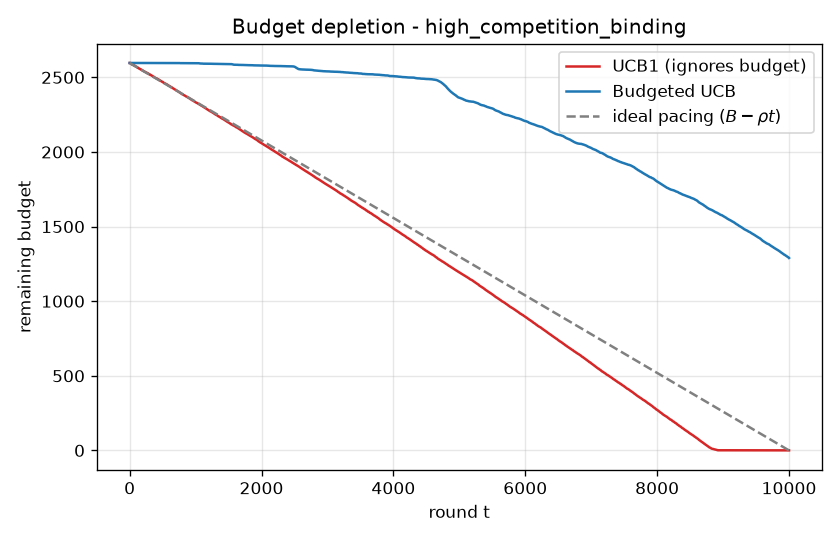
\includegraphics[width=\linewidth]{assets/plots/budget_high_competition_binding.png}
  \caption{\texttt{high\_competition\_binding}}
\end{subfigure}
\hfill
\begin{subfigure}{0.48\textwidth}
  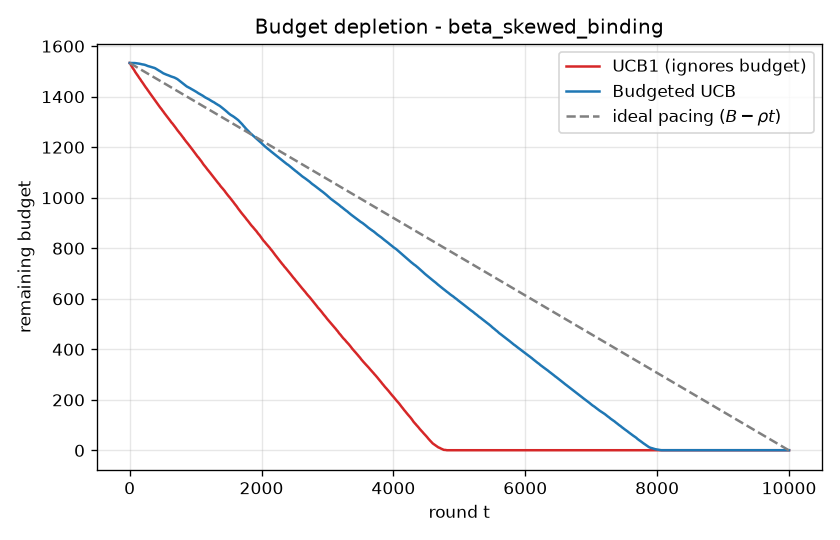
\includegraphics[width=\linewidth]{assets/plots/budget_beta_skewed_binding.png}
  \caption{\texttt{beta\_skewed\_binding}}
\end{subfigure}
\caption{Requirement 1 budget plots, part II.}
\end{figure}

\begin{figure}[p]
\centering
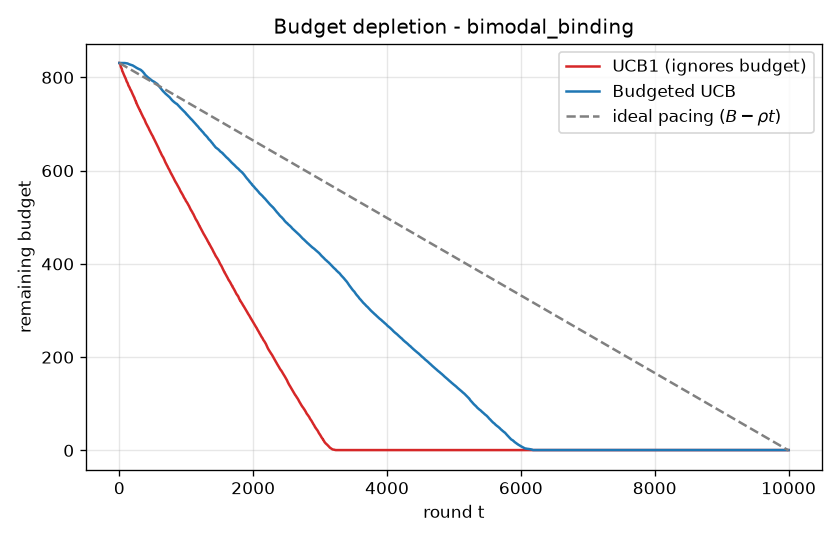
\includegraphics[width=0.48\textwidth]{assets/plots/budget_bimodal_binding.png}
\caption{Requirement 1 budget plot: \texttt{bimodal\_binding}.}
\end{figure}

\begin{figure}[p]
\centering
\begin{subfigure}{0.48\textwidth}
  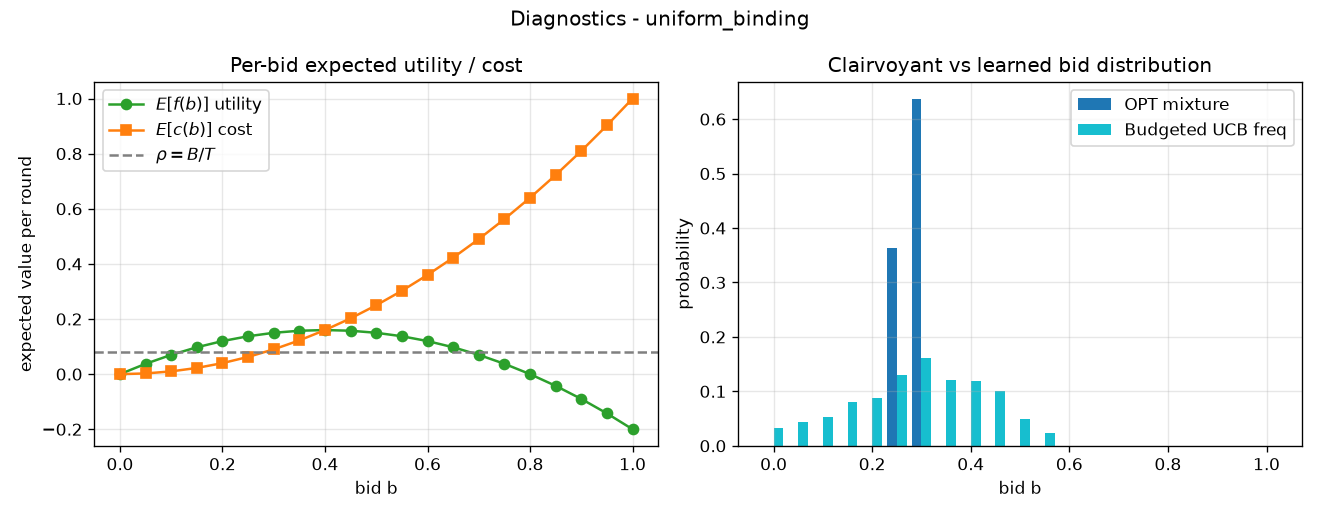
\includegraphics[width=\linewidth]{assets/plots/diagnostics_uniform_binding.png}
  \caption{\texttt{uniform\_binding}}
\end{subfigure}
\hfill
\begin{subfigure}{0.48\textwidth}
  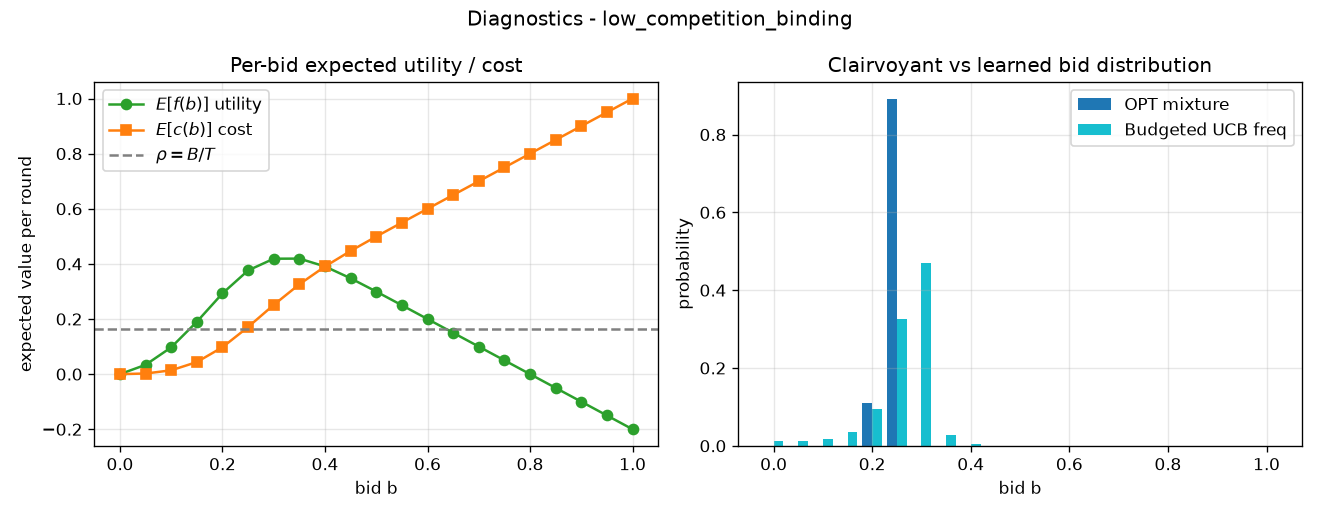
\includegraphics[width=\linewidth]{assets/plots/diagnostics_low_competition_binding.png}
  \caption{\texttt{low\_competition\_binding}}
\end{subfigure}
\caption{Requirement 1 diagnostic plots, part I.}
\end{figure}

\begin{figure}[p]
\centering
\begin{subfigure}{0.48\textwidth}
  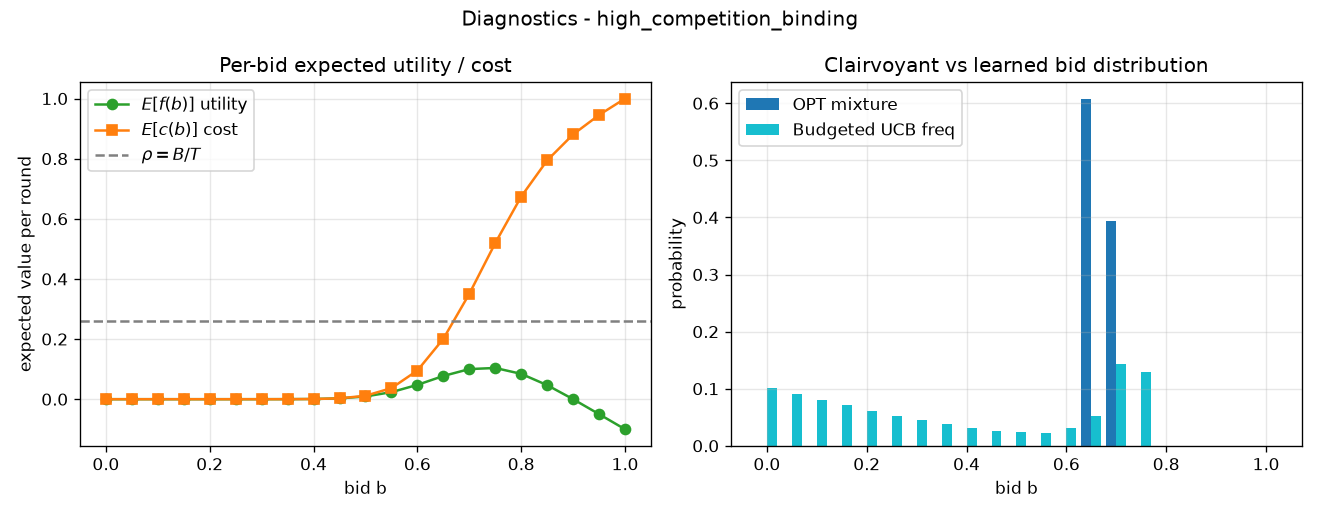
\includegraphics[width=\linewidth]{assets/plots/diagnostics_high_competition_binding.png}
  \caption{\texttt{high\_competition\_binding}}
\end{subfigure}
\hfill
\begin{subfigure}{0.48\textwidth}
  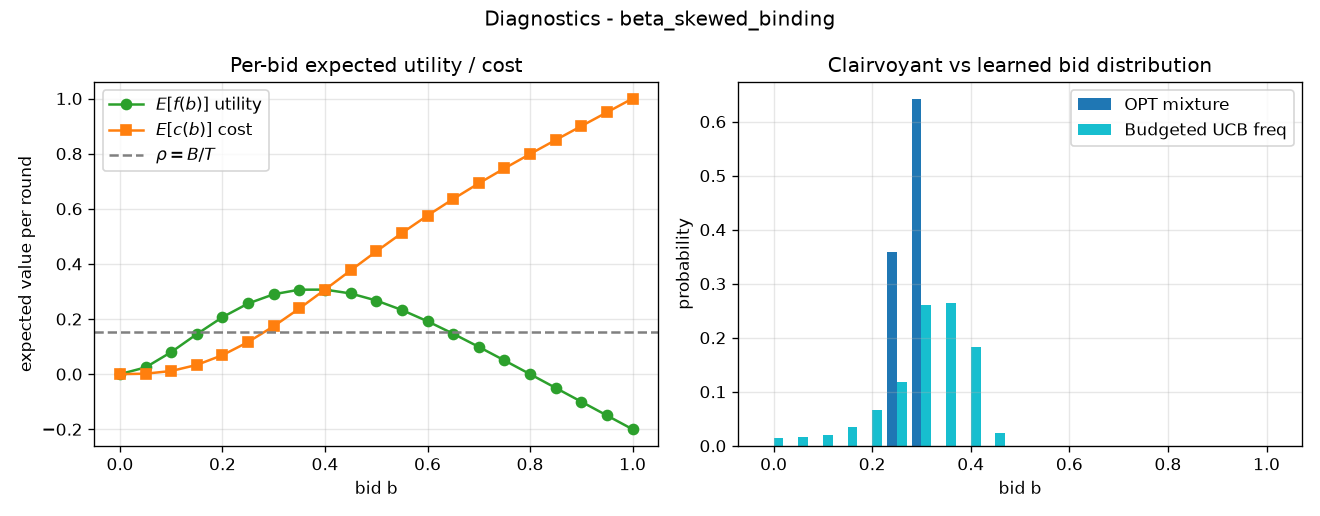
\includegraphics[width=\linewidth]{assets/plots/diagnostics_beta_skewed_binding.png}
  \caption{\texttt{beta\_skewed\_binding}}
\end{subfigure}
\caption{Requirement 1 diagnostic plots, part II.}
\end{figure}

\begin{figure}[p]
\centering
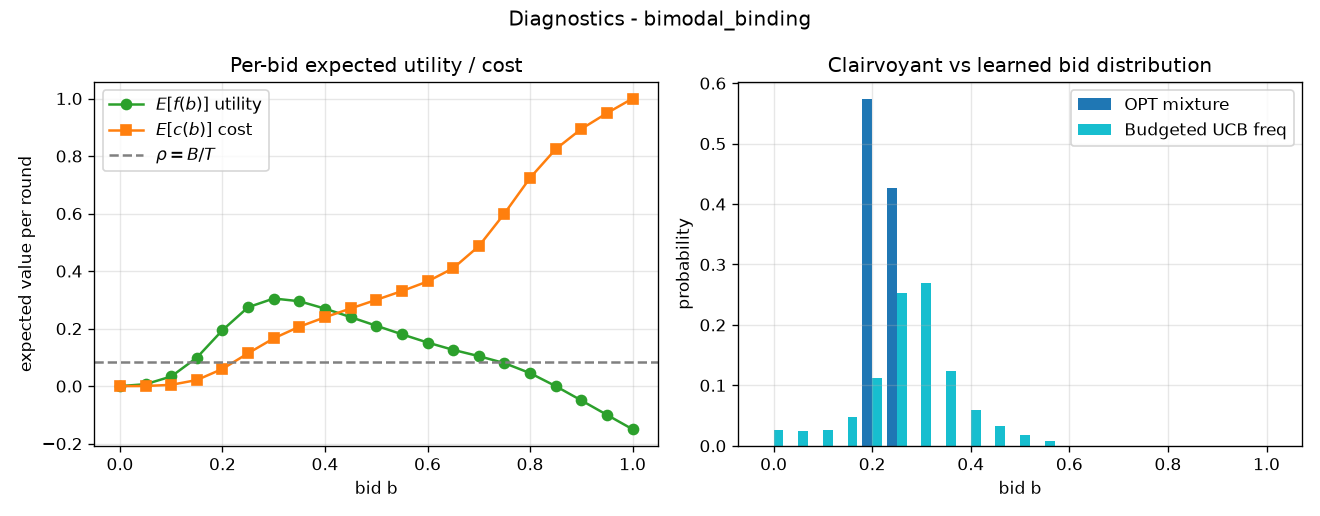
\includegraphics[width=0.48\textwidth]{assets/plots/diagnostics_bimodal_binding.png}
\caption{Requirement 1 diagnostic plot: \texttt{bimodal\_binding}.}
\end{figure}

\begin{figure}[p]
\centering
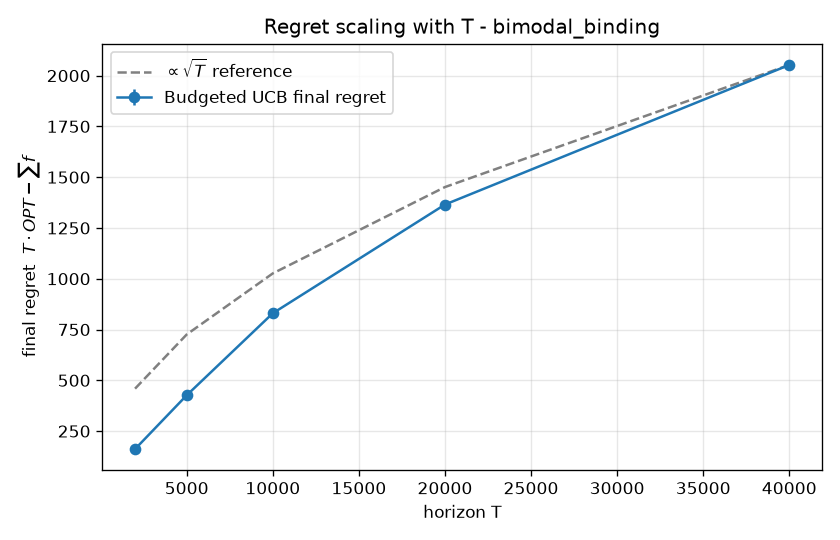
\includegraphics[width=0.70\textwidth]{assets/plots/scaling_regret.png}
\caption{Requirement 1 scaling plot.}
\end{figure}

\subsection{Requirement 2: unique plots}

\begin{figure}[p]
\centering
\begin{subfigure}{0.48\textwidth}
  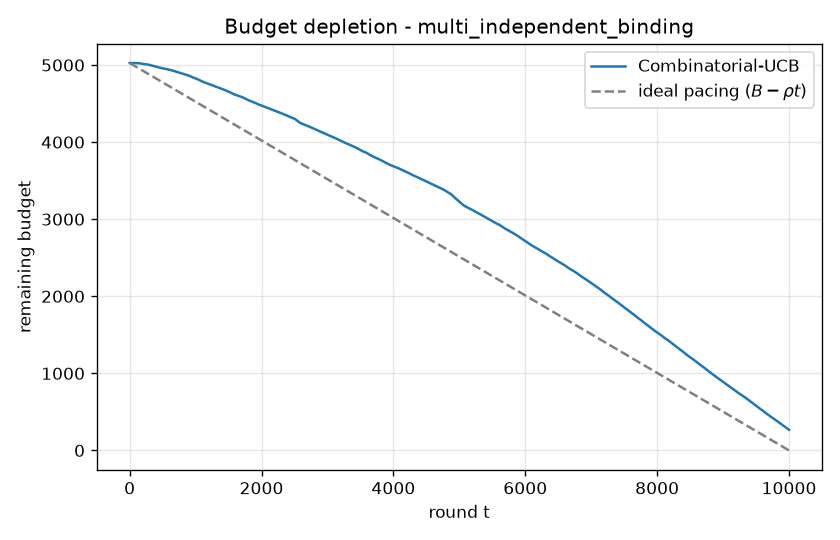
\includegraphics[width=\linewidth]{assets/plots/budget_multi_independent_binding.png}
  \caption{\texttt{multi\_independent\_binding}}
\end{subfigure}
\hfill
\begin{subfigure}{0.48\textwidth}
  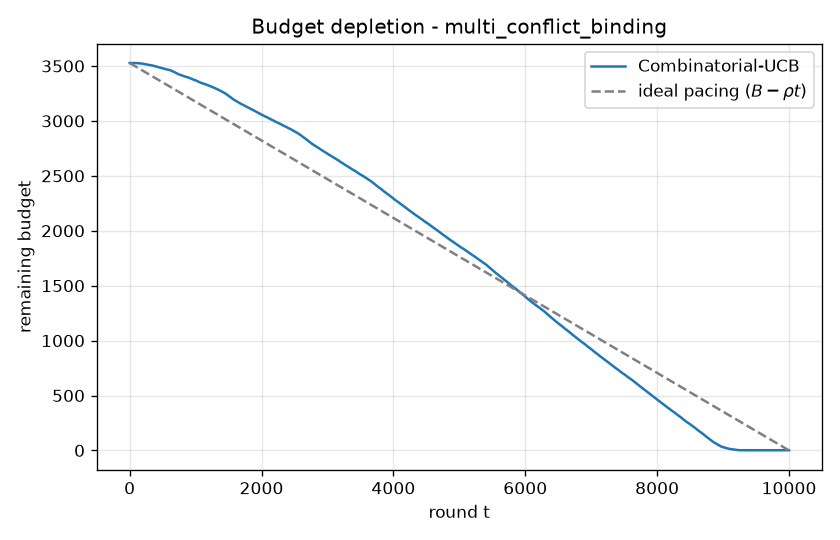
\includegraphics[width=\linewidth]{assets/plots/budget_multi_conflict_binding.png}
  \caption{\texttt{multi\_conflict\_binding}}
\end{subfigure}
\caption{Requirement 2 budget plots, part I.}
\end{figure}

\begin{figure}[p]
\centering
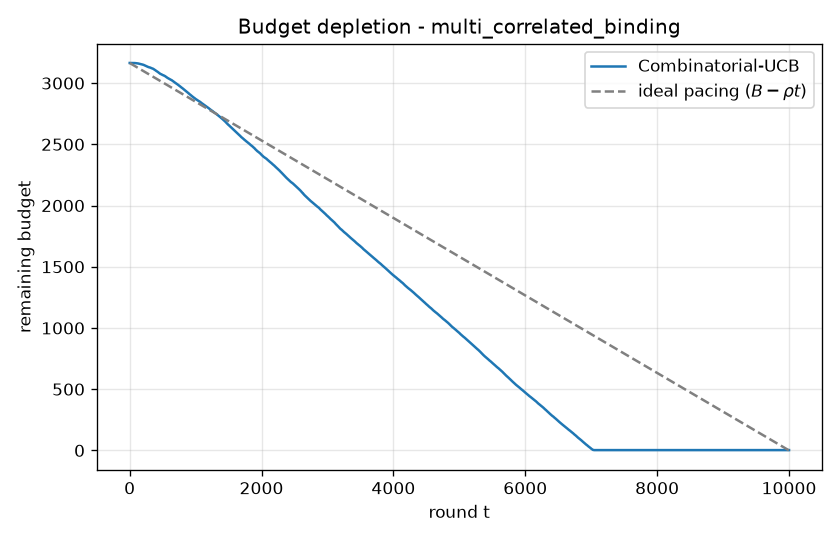
\includegraphics[width=0.48\textwidth]{assets/plots/budget_multi_correlated_binding.png}
\caption{Requirement 2 budget plot: \texttt{multi\_correlated\_binding}.}
\end{figure}

\begin{figure}[p]
\centering
\begin{subfigure}{0.48\textwidth}
  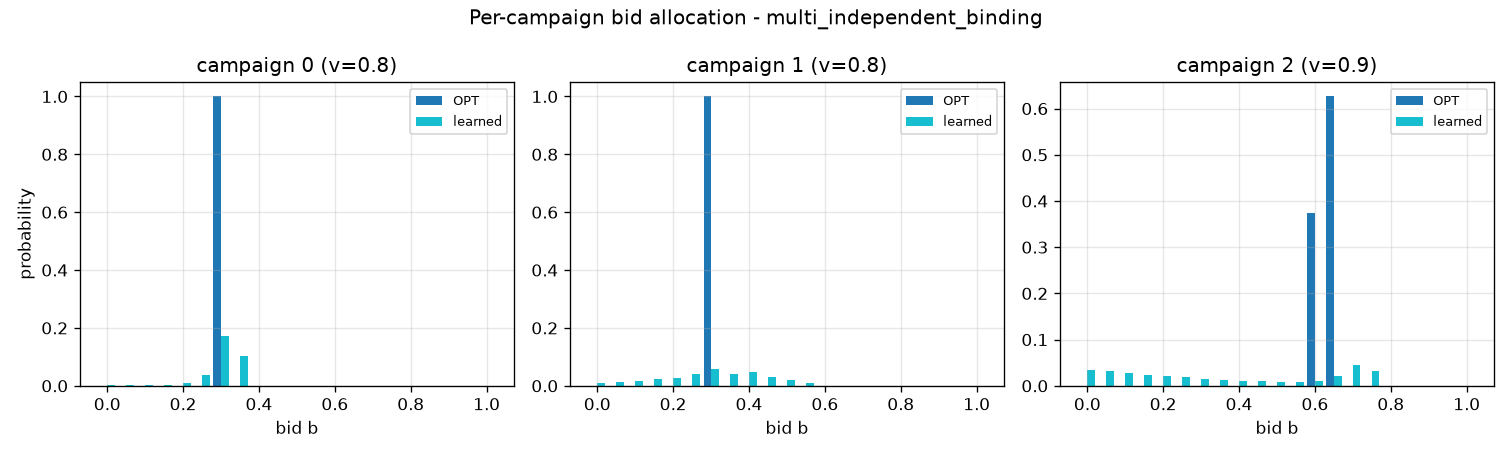
\includegraphics[width=\linewidth]{assets/plots/diagnostics_multi_independent_binding.png}
  \caption{\texttt{multi\_independent\_binding}}
\end{subfigure}
\hfill
\begin{subfigure}{0.48\textwidth}
  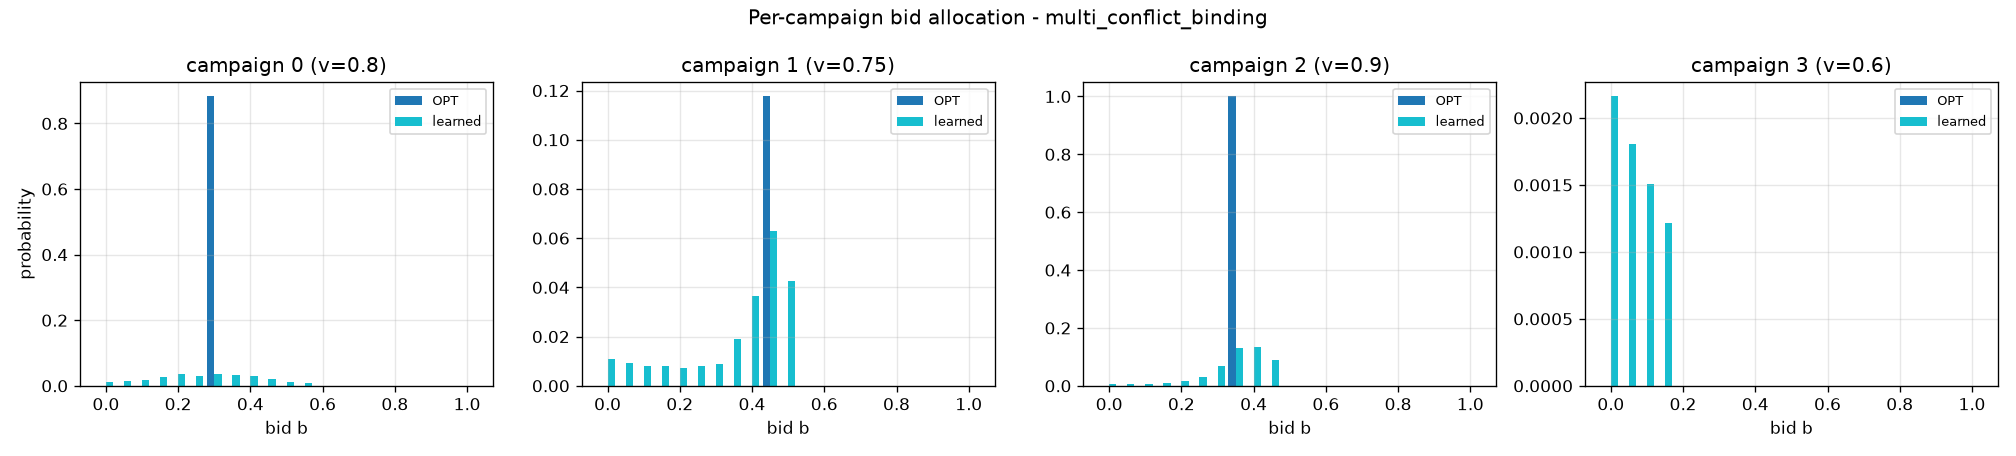
\includegraphics[width=\linewidth]{assets/plots/diagnostics_multi_conflict_binding.png}
  \caption{\texttt{multi\_conflict\_binding}}
\end{subfigure}
\caption{Requirement 2 diagnostics, part I.}
\end{figure}

\begin{figure}[p]
\centering
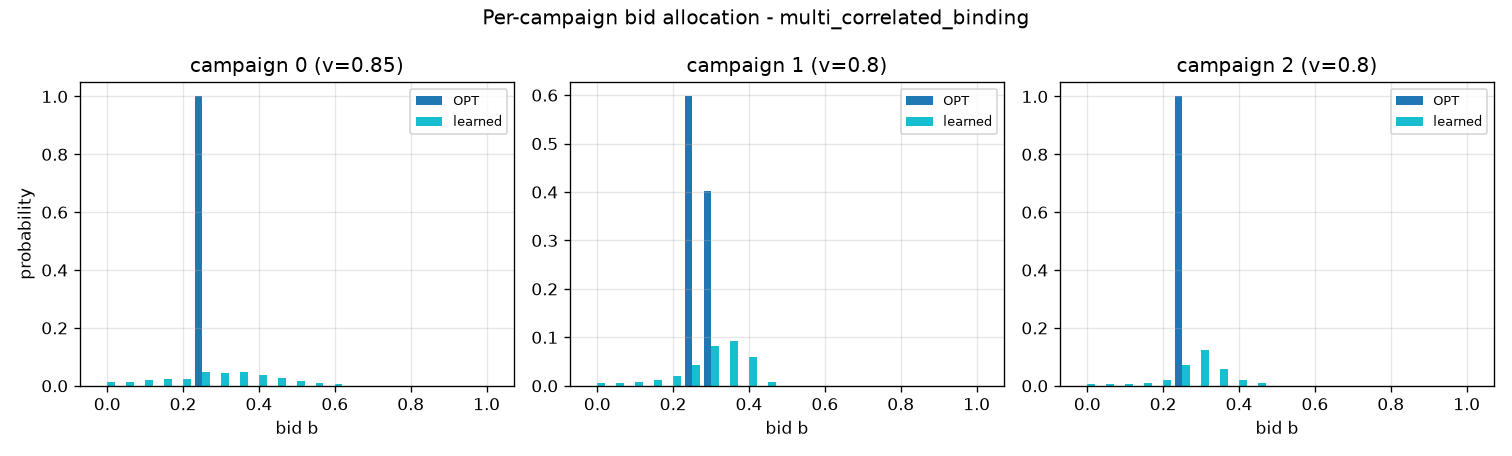
\includegraphics[width=0.48\textwidth]{assets/plots/diagnostics_multi_correlated_binding.png}
\caption{Requirement 2 diagnostic plot: \texttt{multi\_correlated\_binding}.}
\end{figure}

\begin{figure}[p]
\centering
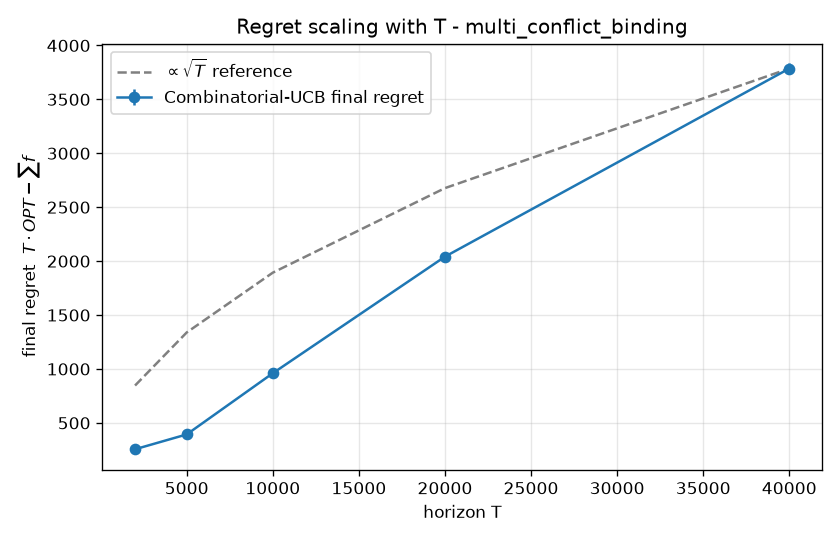
\includegraphics[width=0.70\textwidth]{assets/plots/scaling_regret_multi.png}
\caption{Requirement 2 scaling plot.}
\end{figure}

\subsection{Requirement 3: all plots}

\begin{figure}[p]
\centering
\begin{subfigure}{0.48\textwidth}
  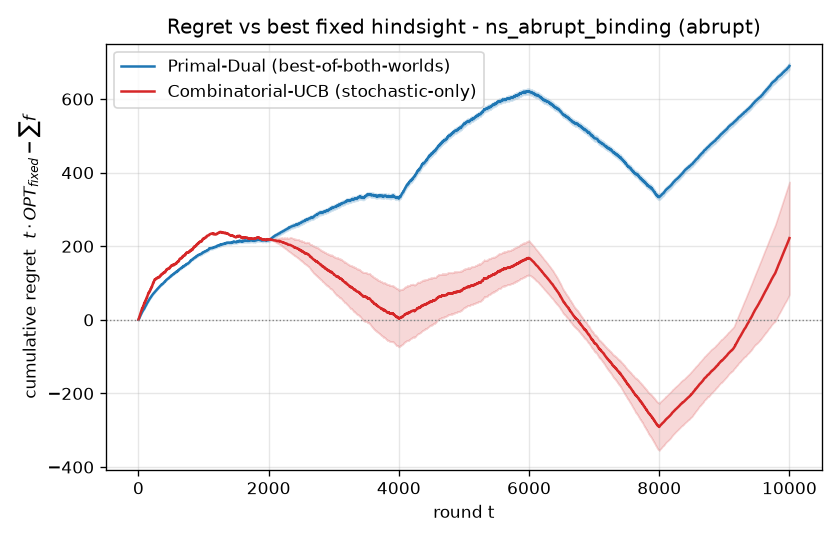
\includegraphics[width=\linewidth]{assets/plots/regret_ns_abrupt_binding.png}
  \caption{\texttt{ns\_abrupt\_binding}}
\end{subfigure}
\hfill
\begin{subfigure}{0.48\textwidth}
  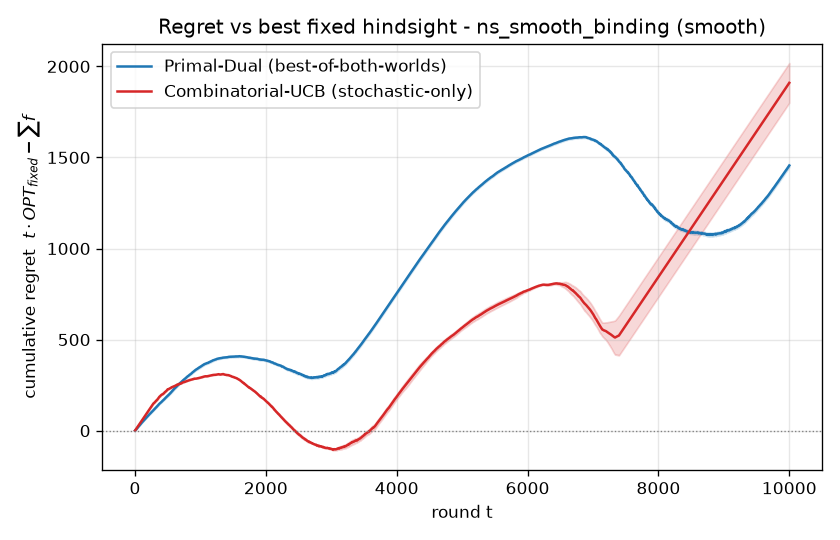
\includegraphics[width=\linewidth]{assets/plots/regret_ns_smooth_binding.png}
  \caption{\texttt{ns\_smooth\_binding}}
\end{subfigure}
\caption{Requirement 3 regret plots, part I.}
\end{figure}

\begin{figure}[p]
\centering
\begin{subfigure}{0.48\textwidth}
  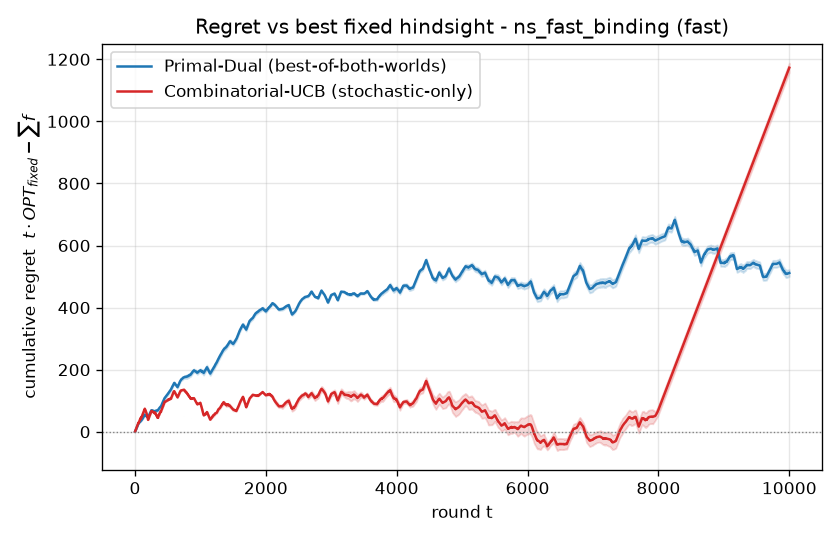
\includegraphics[width=\linewidth]{assets/plots/regret_ns_fast_binding.png}
  \caption{\texttt{ns\_fast\_binding}}
\end{subfigure}
\hfill
\begin{subfigure}{0.48\textwidth}
  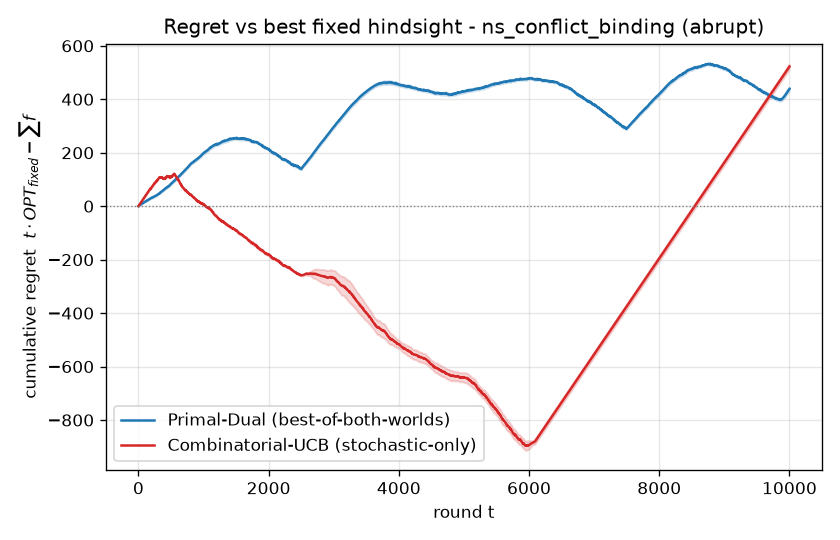
\includegraphics[width=\linewidth]{assets/plots/regret_ns_conflict_binding.png}
  \caption{\texttt{ns\_conflict\_binding}}
\end{subfigure}
\caption{Requirement 3 regret plots, part II.}
\end{figure}

\begin{figure}[p]
\centering
\begin{subfigure}{0.48\textwidth}
  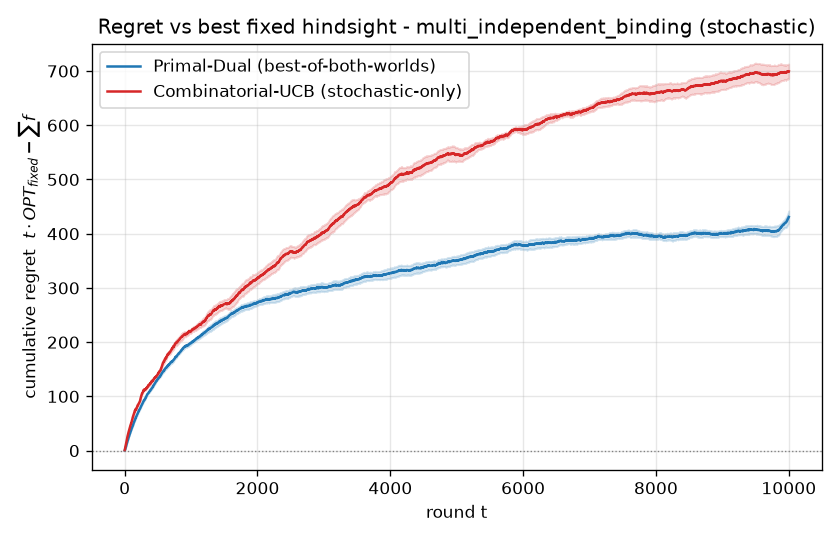
\includegraphics[width=\linewidth]{assets/plots/regret_multi_independent_binding.png}
  \caption{\texttt{multi\_independent\_binding}}
\end{subfigure}
\hfill
\begin{subfigure}{0.48\textwidth}
  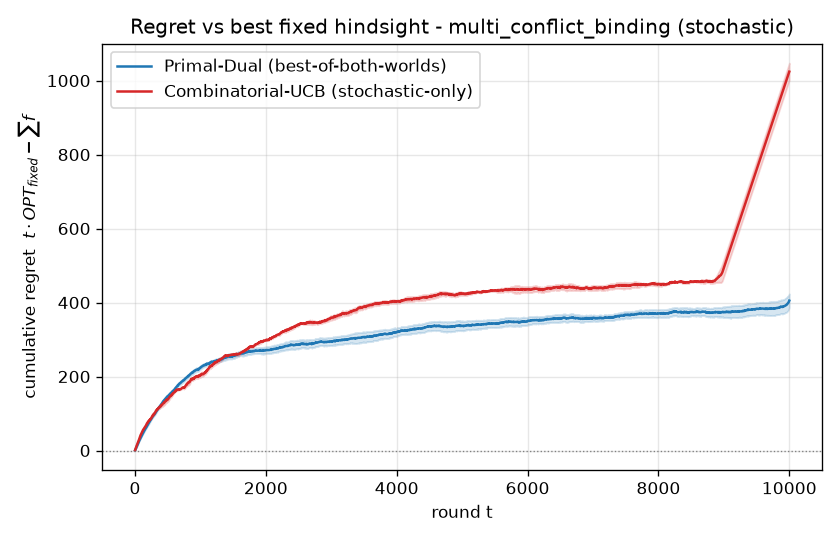
\includegraphics[width=\linewidth]{assets/plots/regret_multi_conflict_binding.png}
  \caption{\texttt{multi\_conflict\_binding}}
\end{subfigure}
\caption{Requirement 3 regret plots on reused stochastic scenarios, part I.}
\end{figure}

\begin{figure}[p]
\centering
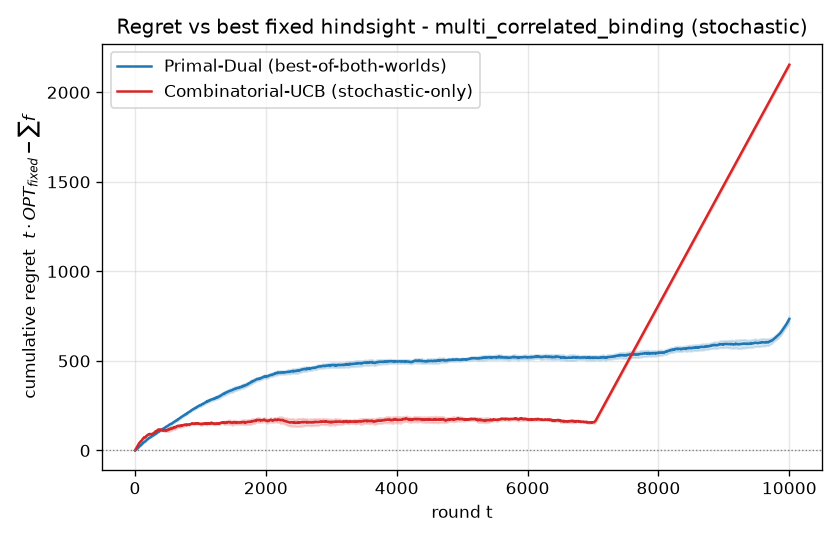
\includegraphics[width=0.48\textwidth]{assets/plots/regret_multi_correlated_binding.png}
\caption{Requirement 3 regret plot on reused stochastic scenario:
\texttt{multi\_correlated\_binding}.}
\end{figure}

\begin{figure}[p]
\centering
\begin{subfigure}{0.48\textwidth}
  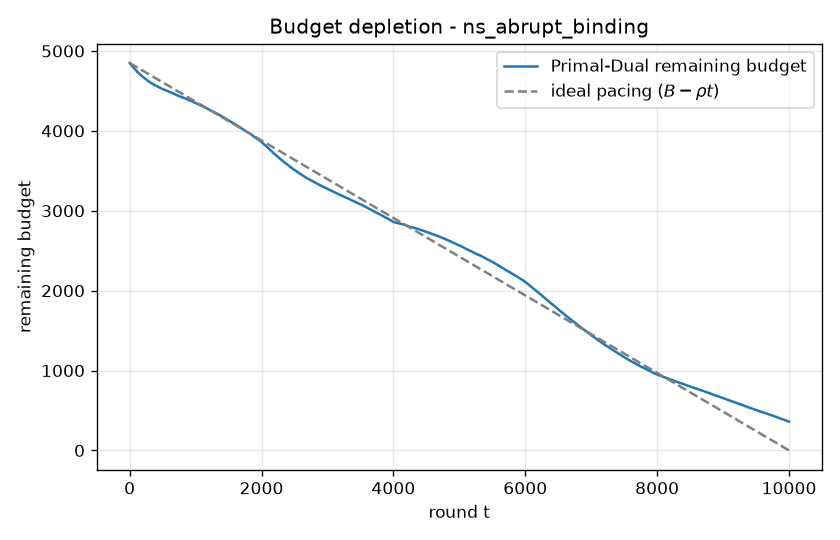
\includegraphics[width=\linewidth]{assets/plots/budget_ns_abrupt_binding.png}
  \caption{\texttt{ns\_abrupt\_binding}}
\end{subfigure}
\hfill
\begin{subfigure}{0.48\textwidth}
  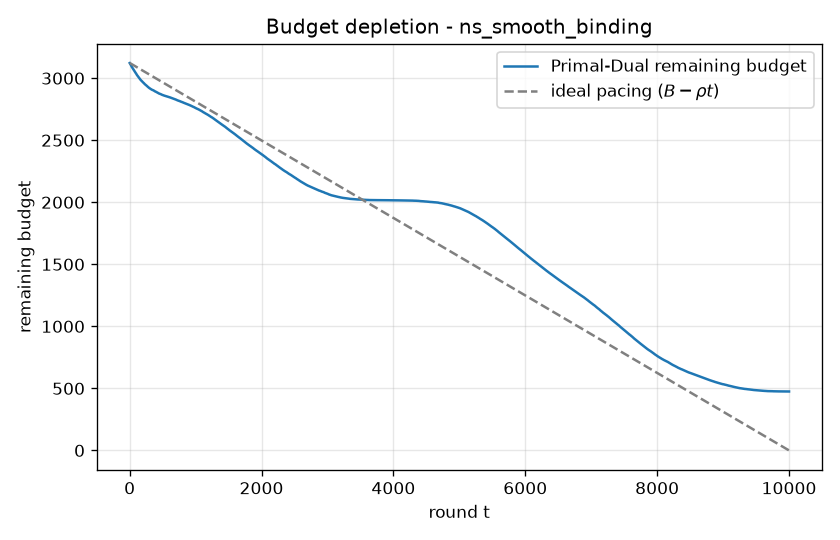
\includegraphics[width=\linewidth]{assets/plots/budget_ns_smooth_binding.png}
  \caption{\texttt{ns\_smooth\_binding}}
\end{subfigure}
\caption{Requirement 3 budget plots, part I.}
\end{figure}

\begin{figure}[p]
\centering
\begin{subfigure}{0.48\textwidth}
  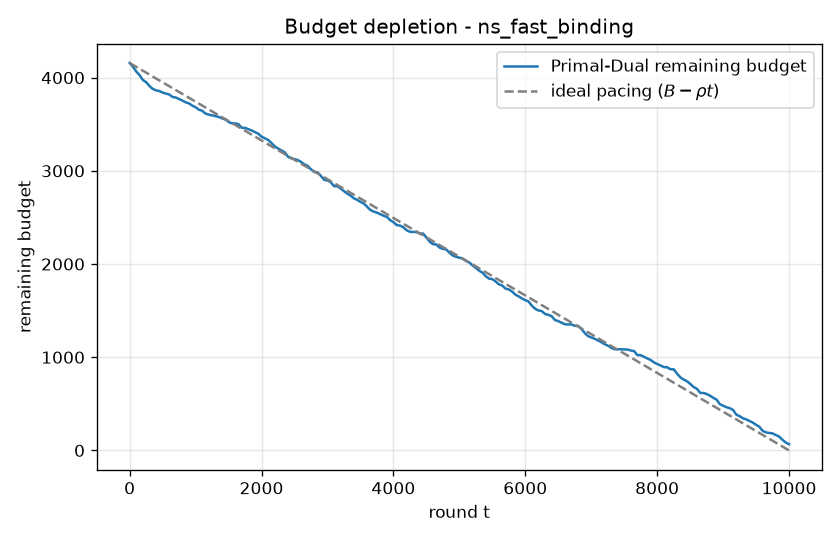
\includegraphics[width=\linewidth]{assets/plots/budget_ns_fast_binding.png}
  \caption{\texttt{ns\_fast\_binding}}
\end{subfigure}
\hfill
\begin{subfigure}{0.48\textwidth}
  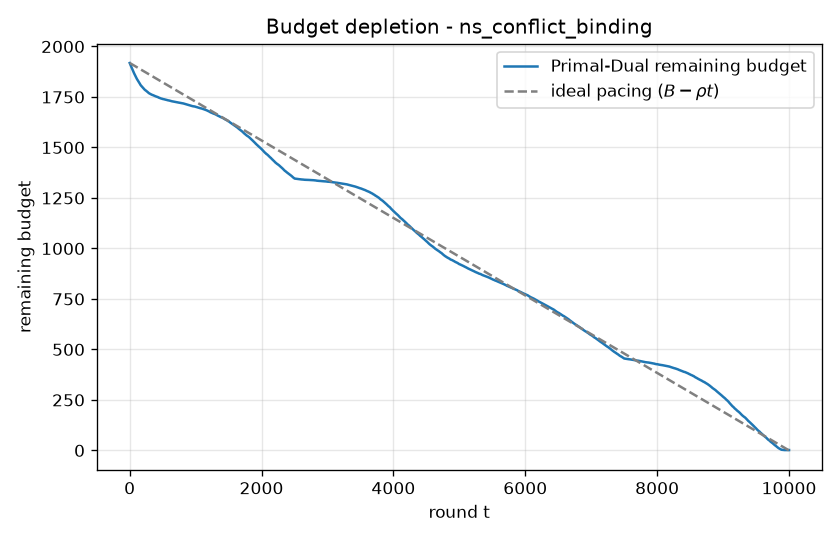
\includegraphics[width=\linewidth]{assets/plots/budget_ns_conflict_binding.png}
  \caption{\texttt{ns\_conflict\_binding}}
\end{subfigure}
\caption{Requirement 3 budget plots, part II.}
\end{figure}

\begin{figure}[p]
\centering
\begin{subfigure}{0.48\textwidth}
  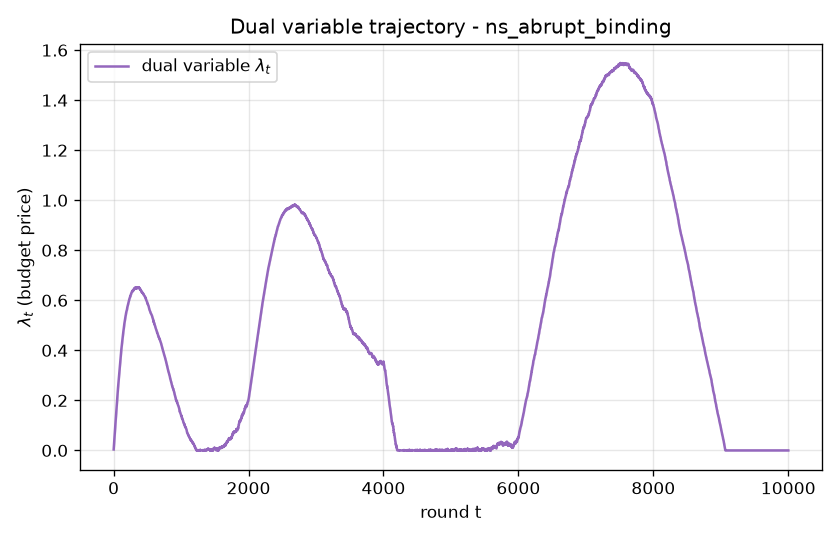
\includegraphics[width=\linewidth]{assets/plots/dual_ns_abrupt_binding.png}
  \caption{\texttt{ns\_abrupt\_binding}}
\end{subfigure}
\hfill
\begin{subfigure}{0.48\textwidth}
  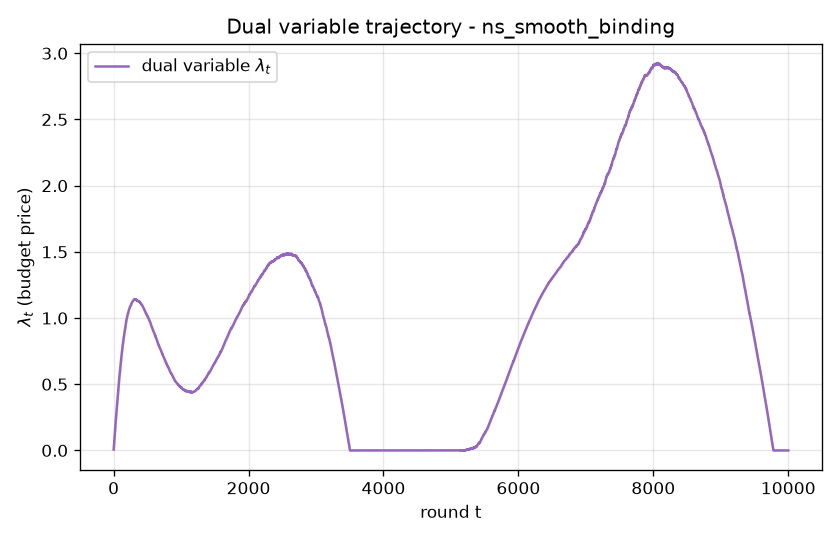
\includegraphics[width=\linewidth]{assets/plots/dual_ns_smooth_binding.png}
  \caption{\texttt{ns\_smooth\_binding}}
\end{subfigure}
\caption{Requirement 3 dual trajectories, part I.}
\end{figure}

\begin{figure}[p]
\centering
\begin{subfigure}{0.48\textwidth}
  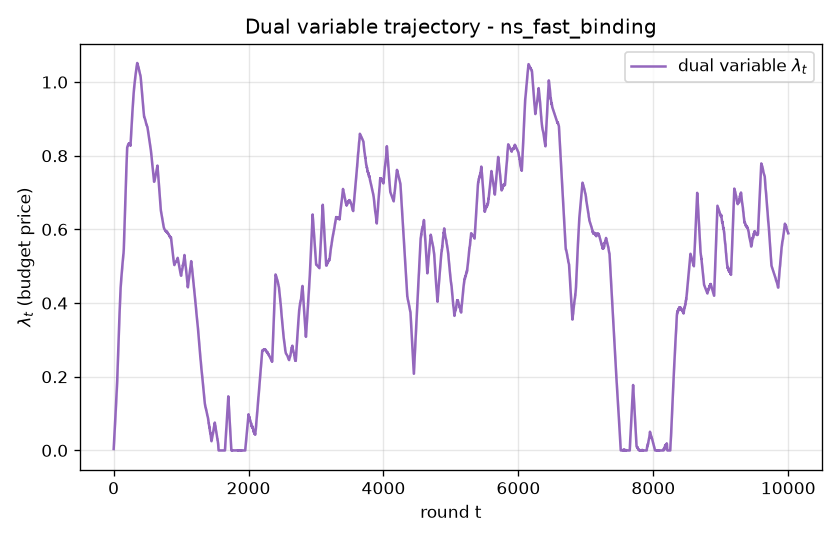
\includegraphics[width=\linewidth]{assets/plots/dual_ns_fast_binding.png}
  \caption{\texttt{ns\_fast\_binding}}
\end{subfigure}
\hfill
\begin{subfigure}{0.48\textwidth}
  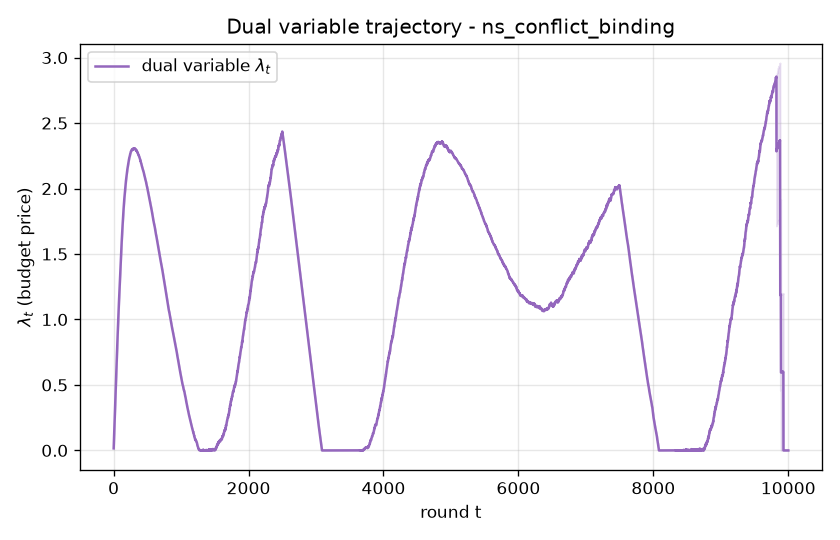
\includegraphics[width=\linewidth]{assets/plots/dual_ns_conflict_binding.png}
  \caption{\texttt{ns\_conflict\_binding}}
\end{subfigure}
\caption{Requirement 3 dual trajectories, part II.}
\end{figure}

\begin{figure}[p]
\centering
\begin{subfigure}{0.62\textwidth}
  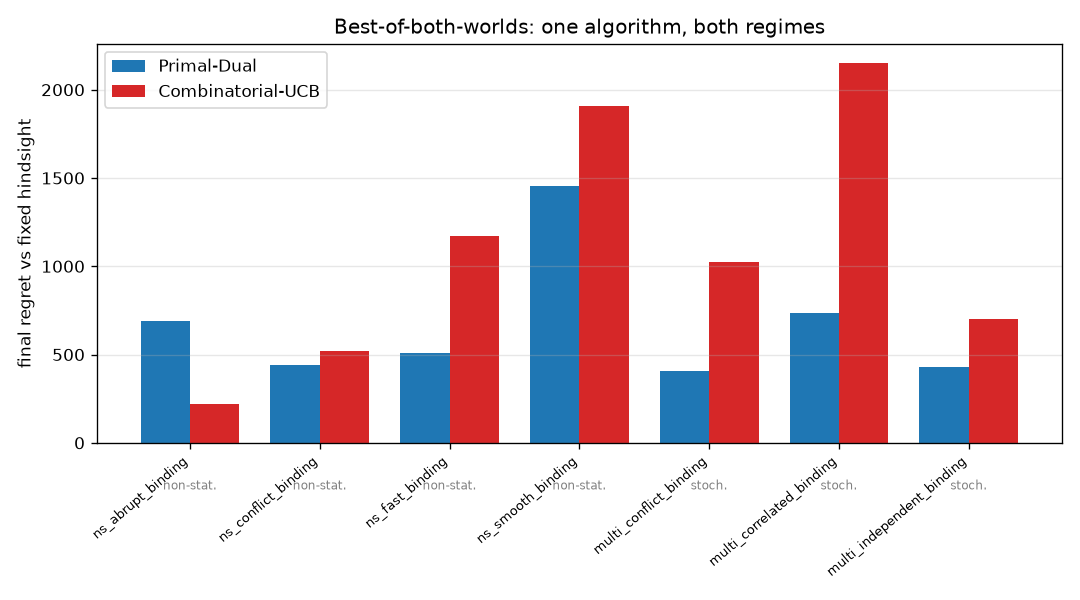
\includegraphics[width=\linewidth]{assets/plots/bobw_summary.png}
  \caption{Best-of-both-worlds summary}
\end{subfigure}

  \vspace{1em}

\begin{subfigure}{0.62\textwidth}
  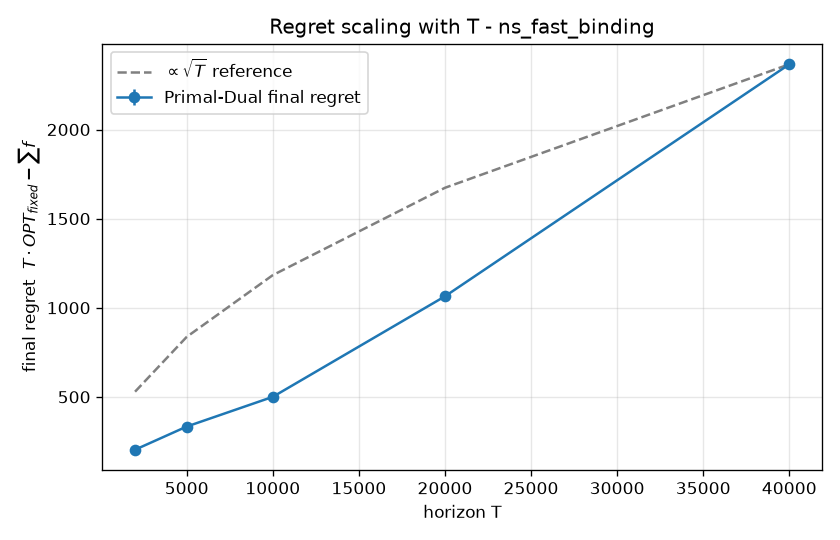
\includegraphics[width=\linewidth]{assets/plots/scaling_regret_pd.png}
  \caption{Scaling experiment}
\end{subfigure}
\caption{Requirement 3 summary figures.}
\end{figure}

\subsection{Requirement 4: all plots}

\begin{figure}[p]
\centering
\begin{subfigure}{0.48\textwidth}
  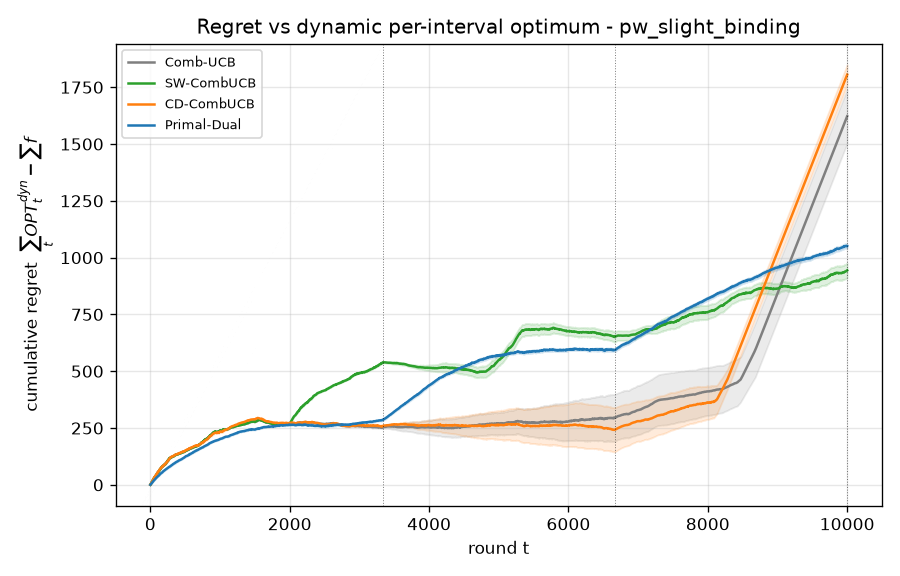
\includegraphics[width=\linewidth]{assets/plots/regret_req4_pw_slight_binding.png}
  \caption{\texttt{pw\_slight\_binding}}
\end{subfigure}
\hfill
\begin{subfigure}{0.48\textwidth}
  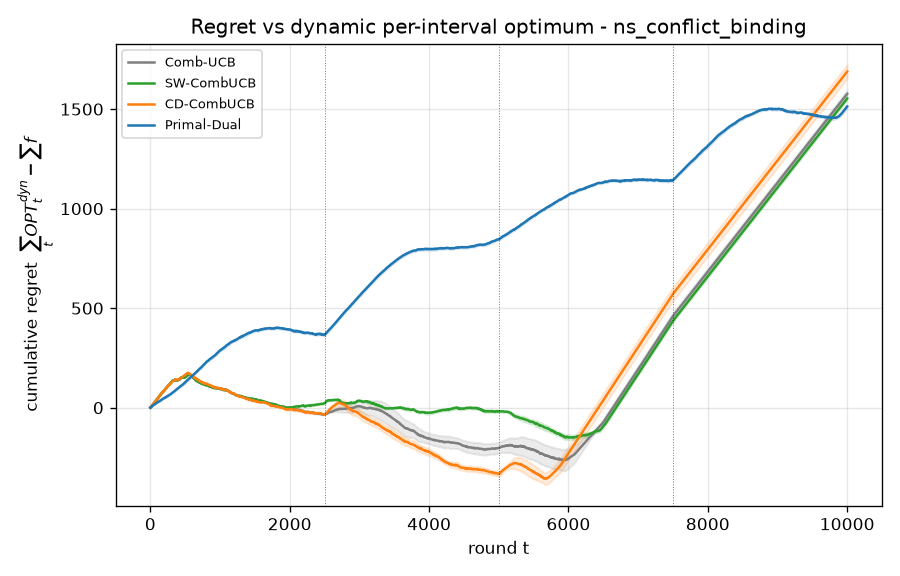
\includegraphics[width=\linewidth]{assets/plots/regret_req4_ns_conflict_binding.png}
  \caption{\texttt{ns\_conflict\_binding}}
\end{subfigure}
\caption{Requirement 4 regret plots, part I.}
\end{figure}

\begin{figure}[p]
\centering
\begin{subfigure}{0.48\textwidth}
  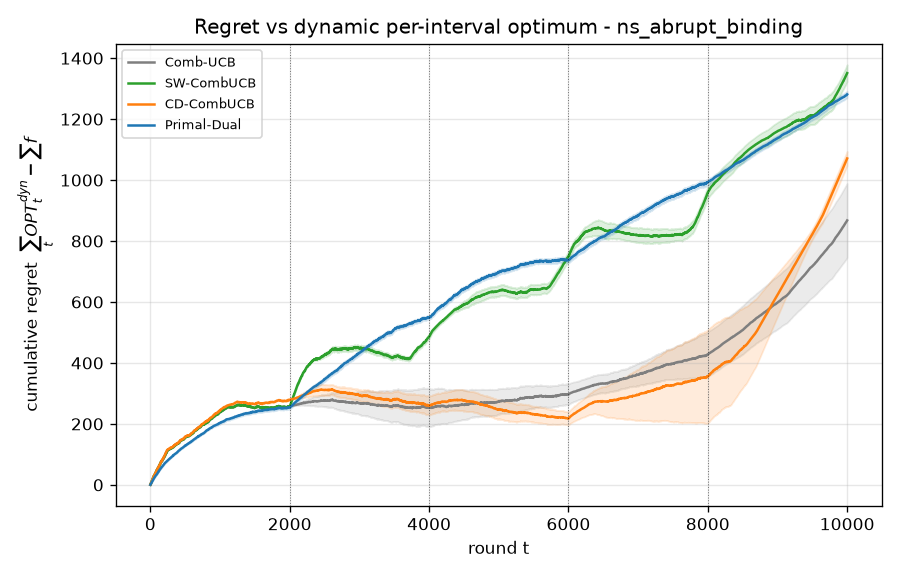
\includegraphics[width=\linewidth]{assets/plots/regret_req4_ns_abrupt_binding.png}
  \caption{\texttt{ns\_abrupt\_binding}}
\end{subfigure}
\hfill
\begin{subfigure}{0.48\textwidth}
  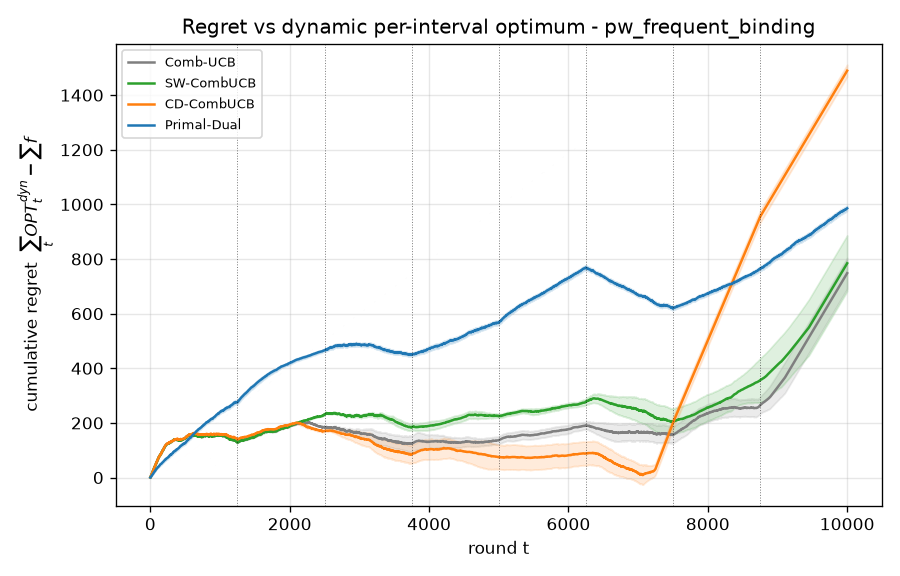
\includegraphics[width=\linewidth]{assets/plots/regret_req4_pw_frequent_binding.png}
  \caption{\texttt{pw\_frequent\_binding}}
\end{subfigure}
\caption{Requirement 4 regret plots, part II.}
\end{figure}

\begin{figure}[p]
\centering
\begin{subfigure}{0.48\textwidth}
  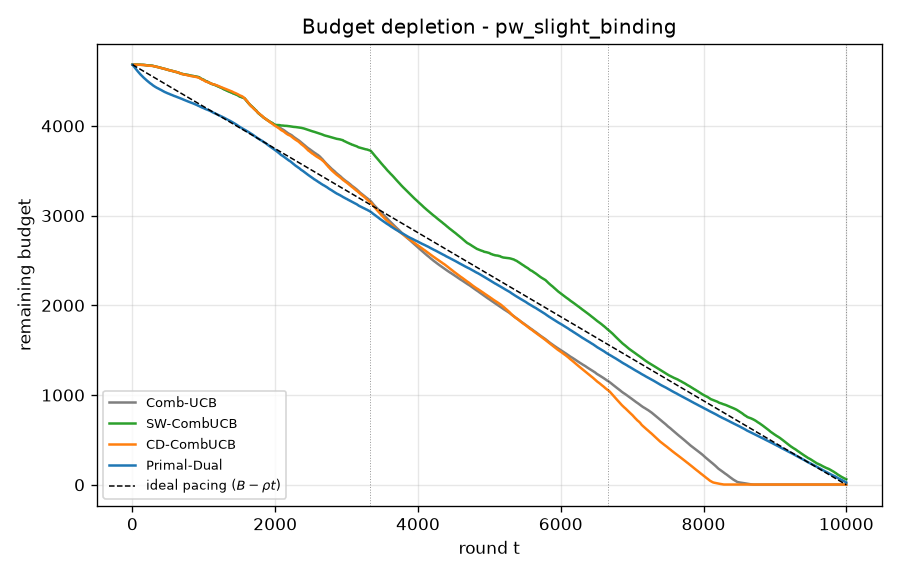
\includegraphics[width=\linewidth]{assets/plots/budget_req4_pw_slight_binding.png}
  \caption{\texttt{pw\_slight\_binding}}
\end{subfigure}
\hfill
\begin{subfigure}{0.48\textwidth}
  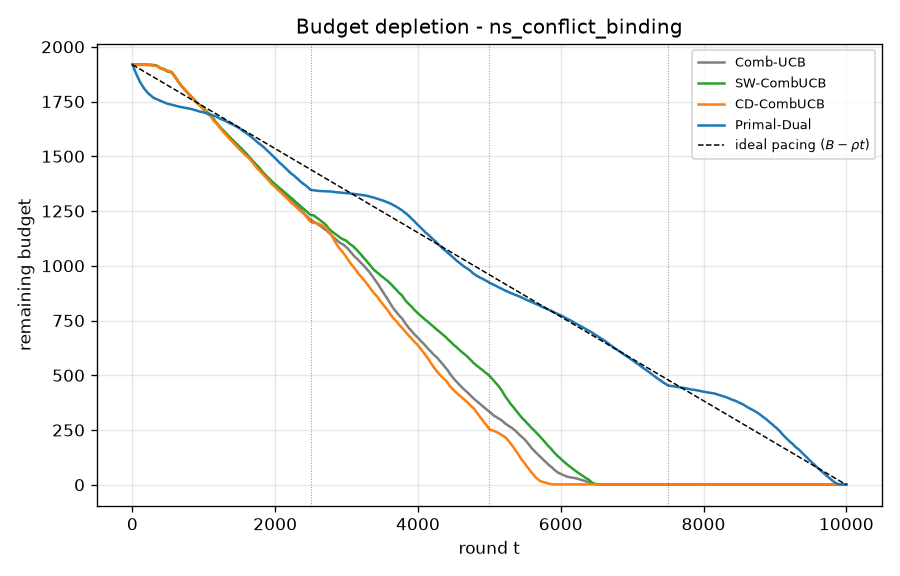
\includegraphics[width=\linewidth]{assets/plots/budget_req4_ns_conflict_binding.png}
  \caption{\texttt{ns\_conflict\_binding}}
\end{subfigure}
\caption{Requirement 4 budget plots, part I.}
\end{figure}

\begin{figure}[p]
\centering
\begin{subfigure}{0.48\textwidth}
  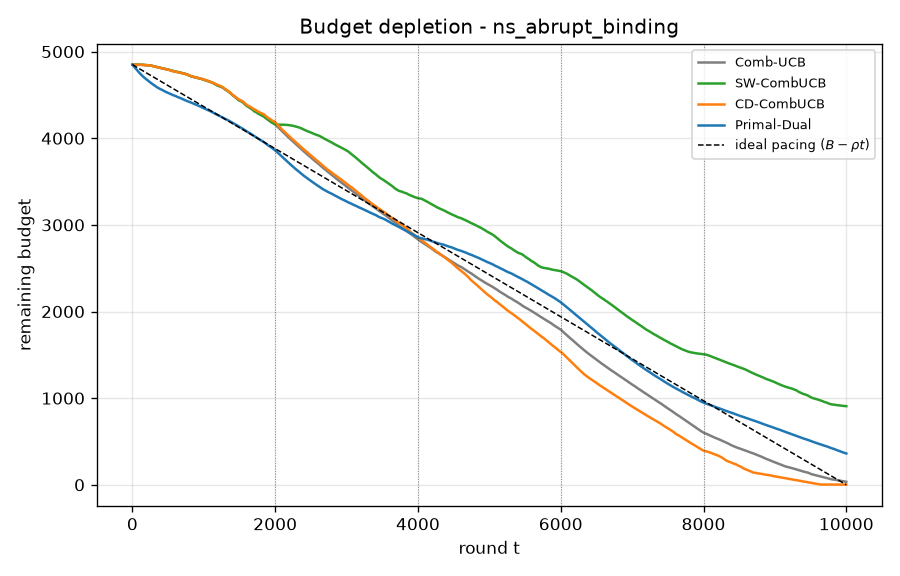
\includegraphics[width=\linewidth]{assets/plots/budget_req4_ns_abrupt_binding.png}
  \caption{\texttt{ns\_abrupt\_binding}}
\end{subfigure}
\hfill
\begin{subfigure}{0.48\textwidth}
  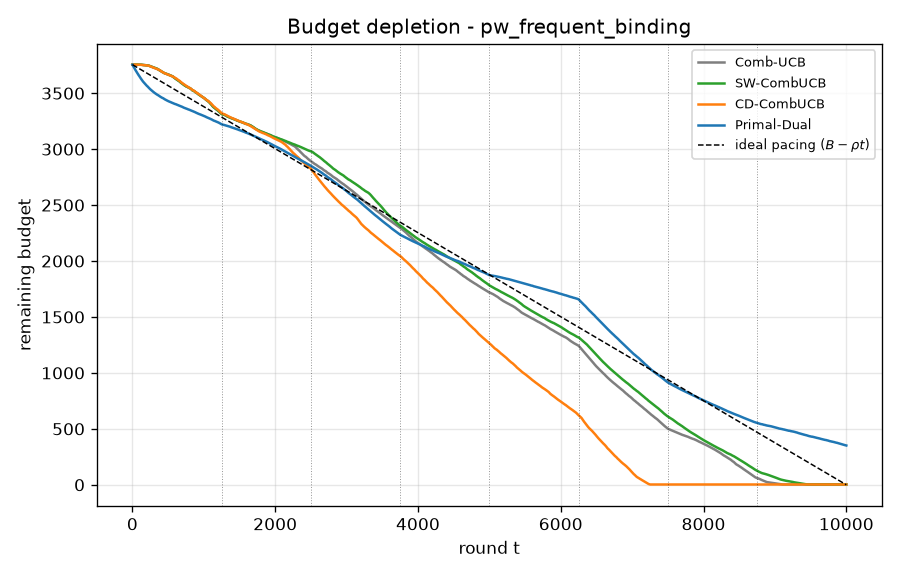
\includegraphics[width=\linewidth]{assets/plots/budget_req4_pw_frequent_binding.png}
  \caption{\texttt{pw\_frequent\_binding}}
\end{subfigure}
\caption{Requirement 4 budget plots, part II.}
\end{figure}

\begin{figure}[p]
\centering
\begin{subfigure}{0.62\textwidth}
  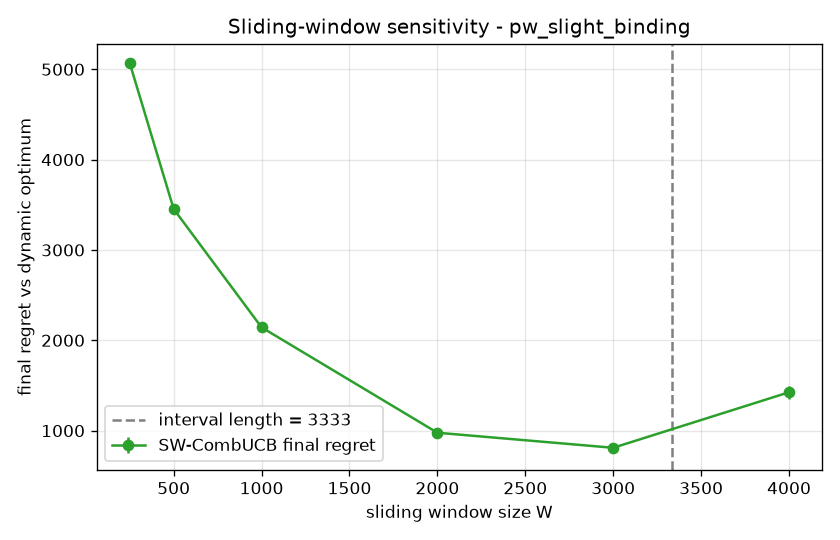
\includegraphics[width=\linewidth]{assets/plots/window_sensitivity.png}
  \caption{Window sensitivity}
\end{subfigure}

  \vspace{1em}

\begin{subfigure}{0.62\textwidth}
  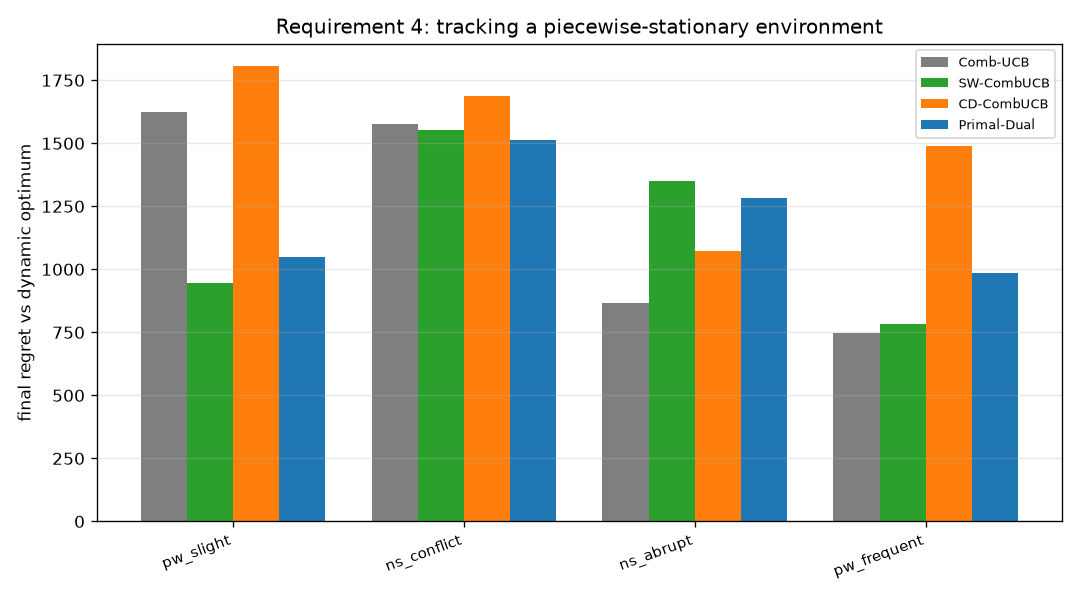
\includegraphics[width=\linewidth]{assets/plots/req4_summary.png}
  \caption{Requirement 4 summary}
\end{subfigure}
\caption{Requirement 4 summary figures.}
\end{figure}

\end{document}
